% !TEX root = thesis-ex.tex

The energy required to dissociate partons increases the further apart they are as a consequence of color confinement.
If the energy with which they are flying apart is greater than the energy required to separate them, it becomes more favorable to produce a quark-antiquark ($q\bar{q}$) pair.
This process of $q \bar{q}$ production continues recursively until it is not energetically favorable to do so, with the end result being conical sprays of hadrons called jets.
This picture is qualitatively supported by Lattice QCD~\cite{PhysRevD.71.114513}. 
A schematic of this process is shown in Figure~\ref{fig:qqbar_to_jet}.
Because of their color charge, gluon led jets have a softer fragmentation and result in more particles carrying lesser energy as compared to quark led jets \cite{Abbiendi:1999pi}.

\begin{figure}[htbp]
\begin{center}
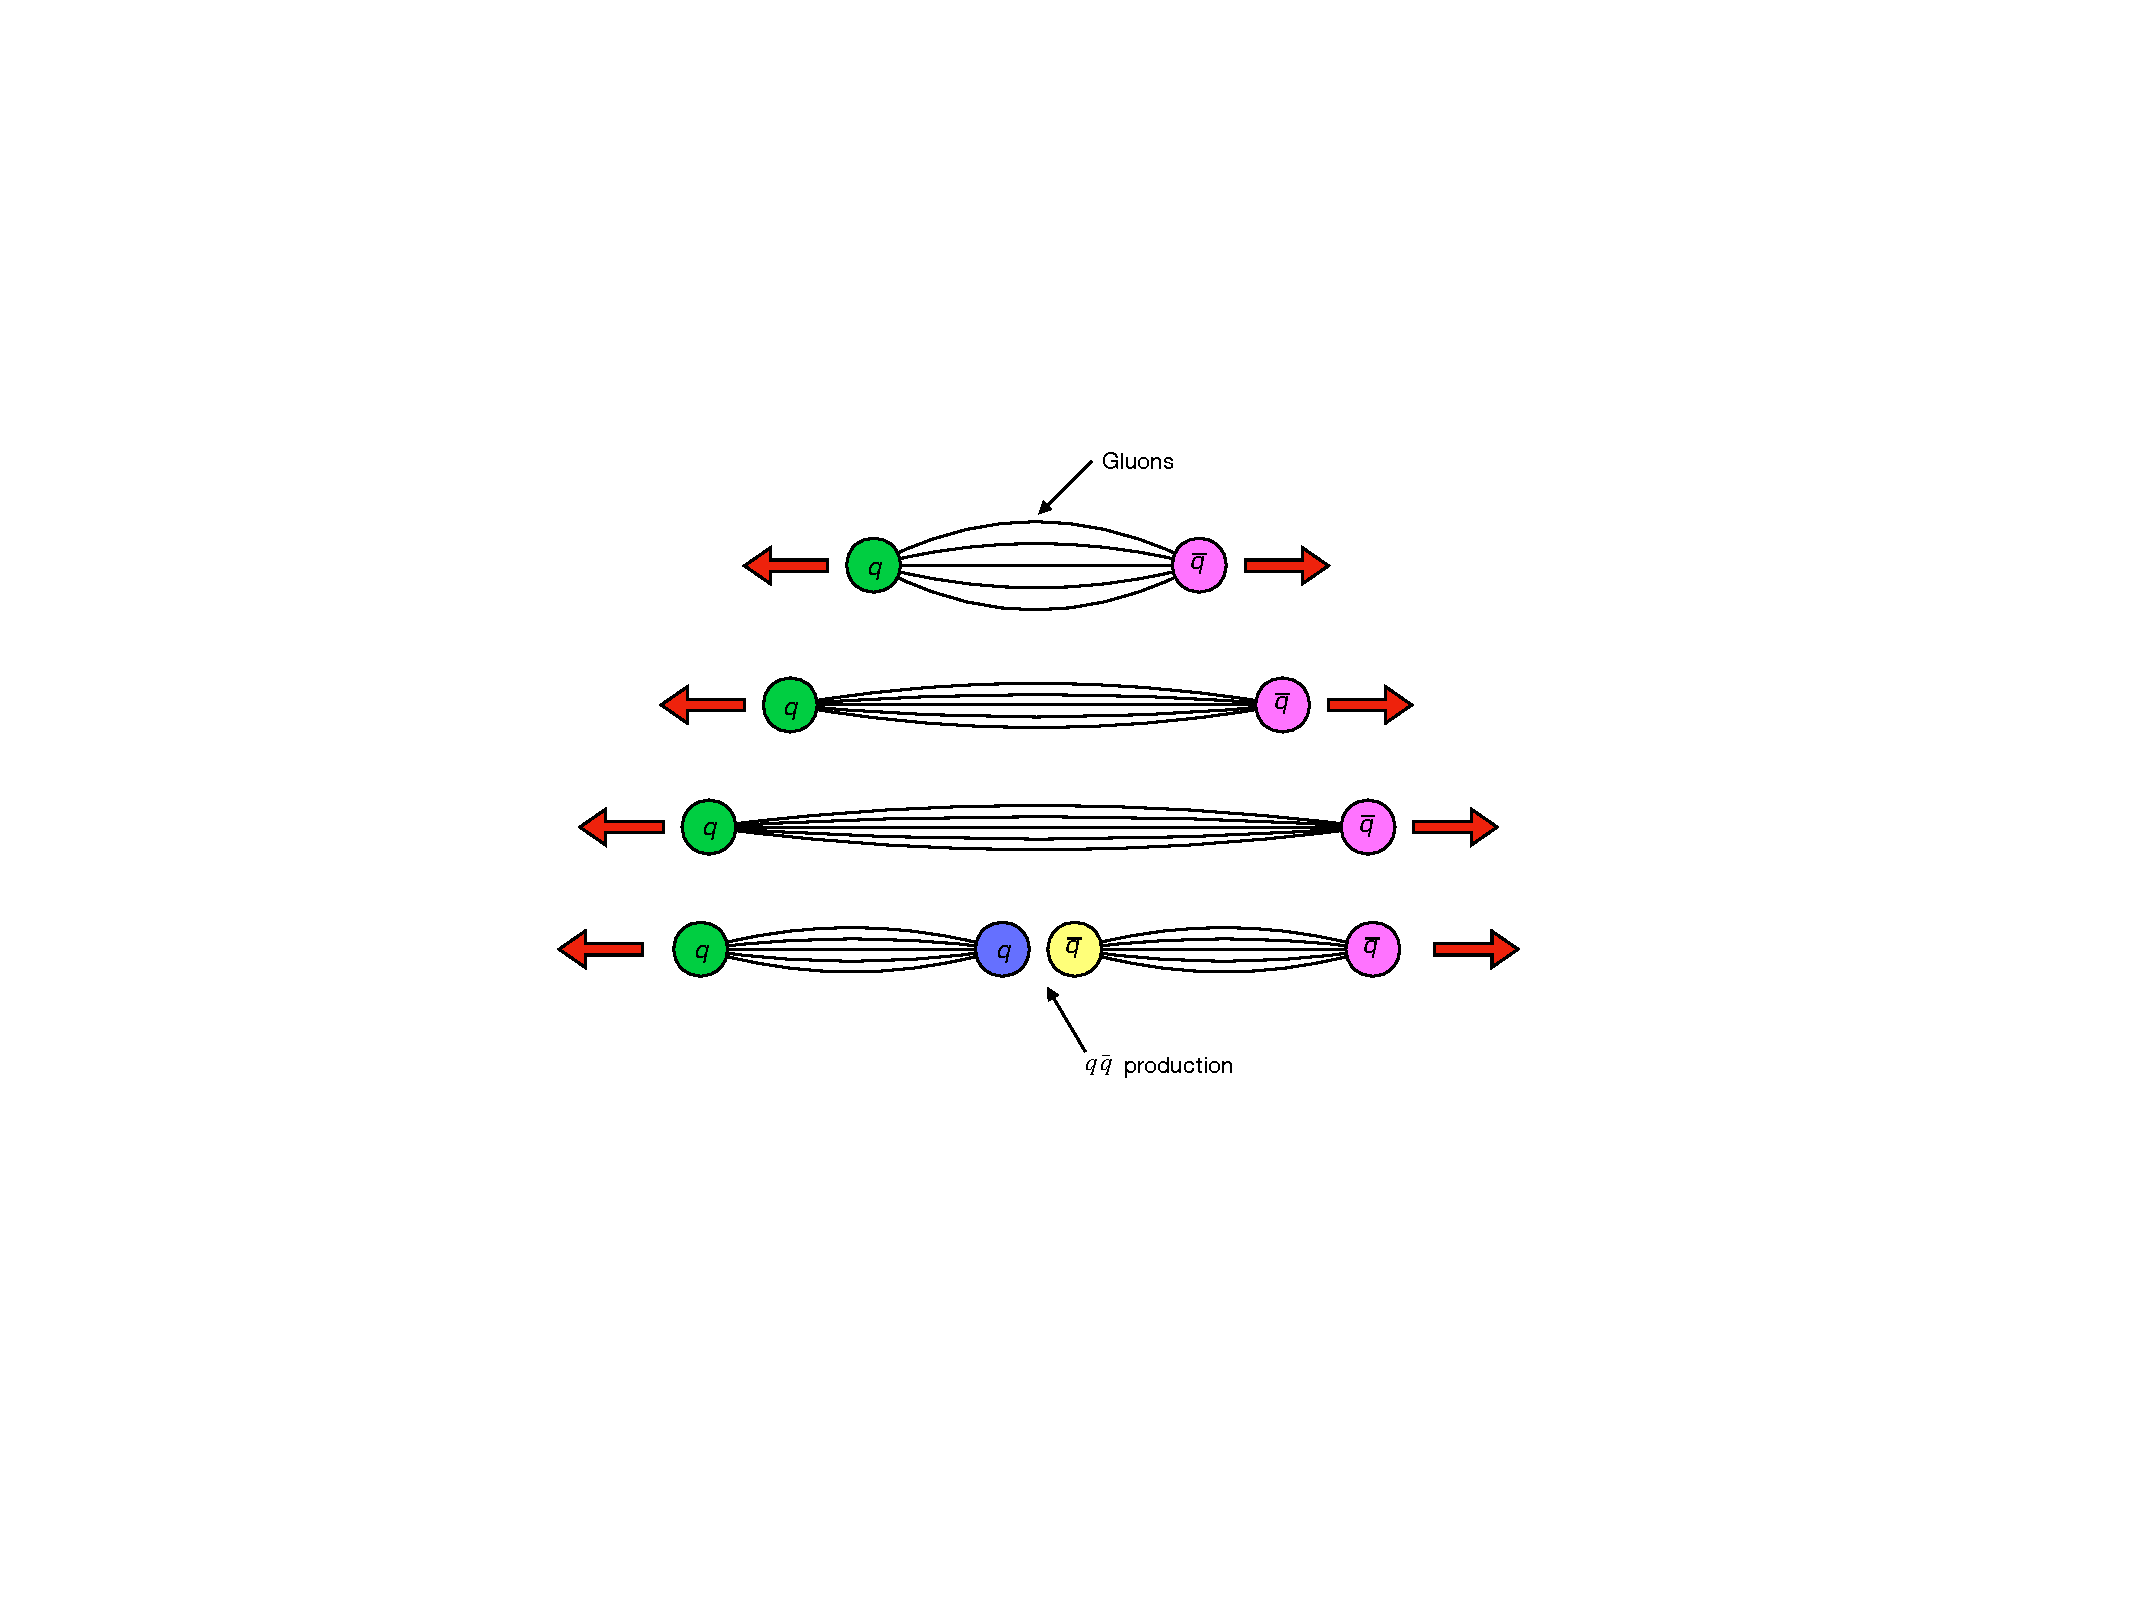
\includegraphics[width=0.55\textwidth]{figures/theory/qqbar_to_jet}
\caption{A schematic of how jets are produced from a hard process involving $q \bar{q}$. The gluonic flux tubes build up and break as the quarks gain energy, and result in the formation of new \qqbar\ pairs.}
\label{fig:qqbar_to_jet}
\end{center}
\end{figure}

\subsection{Jets in $e^+ e^-$ collisions}
The simplest process that can be used to study jets is the process $e^+ e^- \rightarrow q \bar{q} \rightarrow 2 \text{ jets}$.
The electron and positron annihilates to produce a photon that can decay into a $q \bar{q}$ pair, that hadronize and form jets.
In fact, this was the process that provided experiment evidence of jets at SPEAR (Stanford Positron Electron Accelerating Ring) at SLAC in 1975, where it was observed that the distribution of final state hadrons was not isotropic \cite{PhysRevLett.35.1609, PhysRevD.26.991}.
Analyses of these distributions showed that they were associated with spin $1/2$ quarks.
Jets in $e^+ e^-$ collisions further provided the first indirect evidence of gluons when three jet events were observed in the $\Upsilon \rightarrow ggg$ decay \cite{Berger:1978rr, Berger:1979cj}. 
At the Large Electron-Positron Collider (LEP), higher collision energies allowed the $e^+ e^- \rightarrow Z^0 \rightarrow q \bar{q}$ process.
In these processes, to leading order, the \qqbar\ pair evolved via gluon radiation before converting to hadrons \cite{Mueller_1991}, allowing for events with more than two jets.
Jet production in \epm\ collisions is also one of the best ways to test the validity of perturbative QCD \cite{Kramer:1986mc}.

%%%%%%%%%%%%%%%%%%%
\subsection{Jets in $pp$ collisions}
Jet production in a vacuum is well described in context of perturbative QCD \cite{Sjostrand:2007gs}.
Processes involving large momentum transfers like high \pt\ hadron production are shown in Figure~\ref{fig:feynman_jet}
\footnote{In the context of a particle collision, the \pt\ of a particle is the momentum it carries in a direction perpendicular to the beam axis.
It is given by $\pt = |p| \sin\theta$ where $\theta$ is the angle of the particle with respect to the beam axis.
The rapidity $y$ is related to an outgoing particles momentum along the beam axis, and is given by $y = 1/2 \ln[(E+p_z) / (E-p_z)]$}.

\begin{figure}[htbp]
\begin{center}
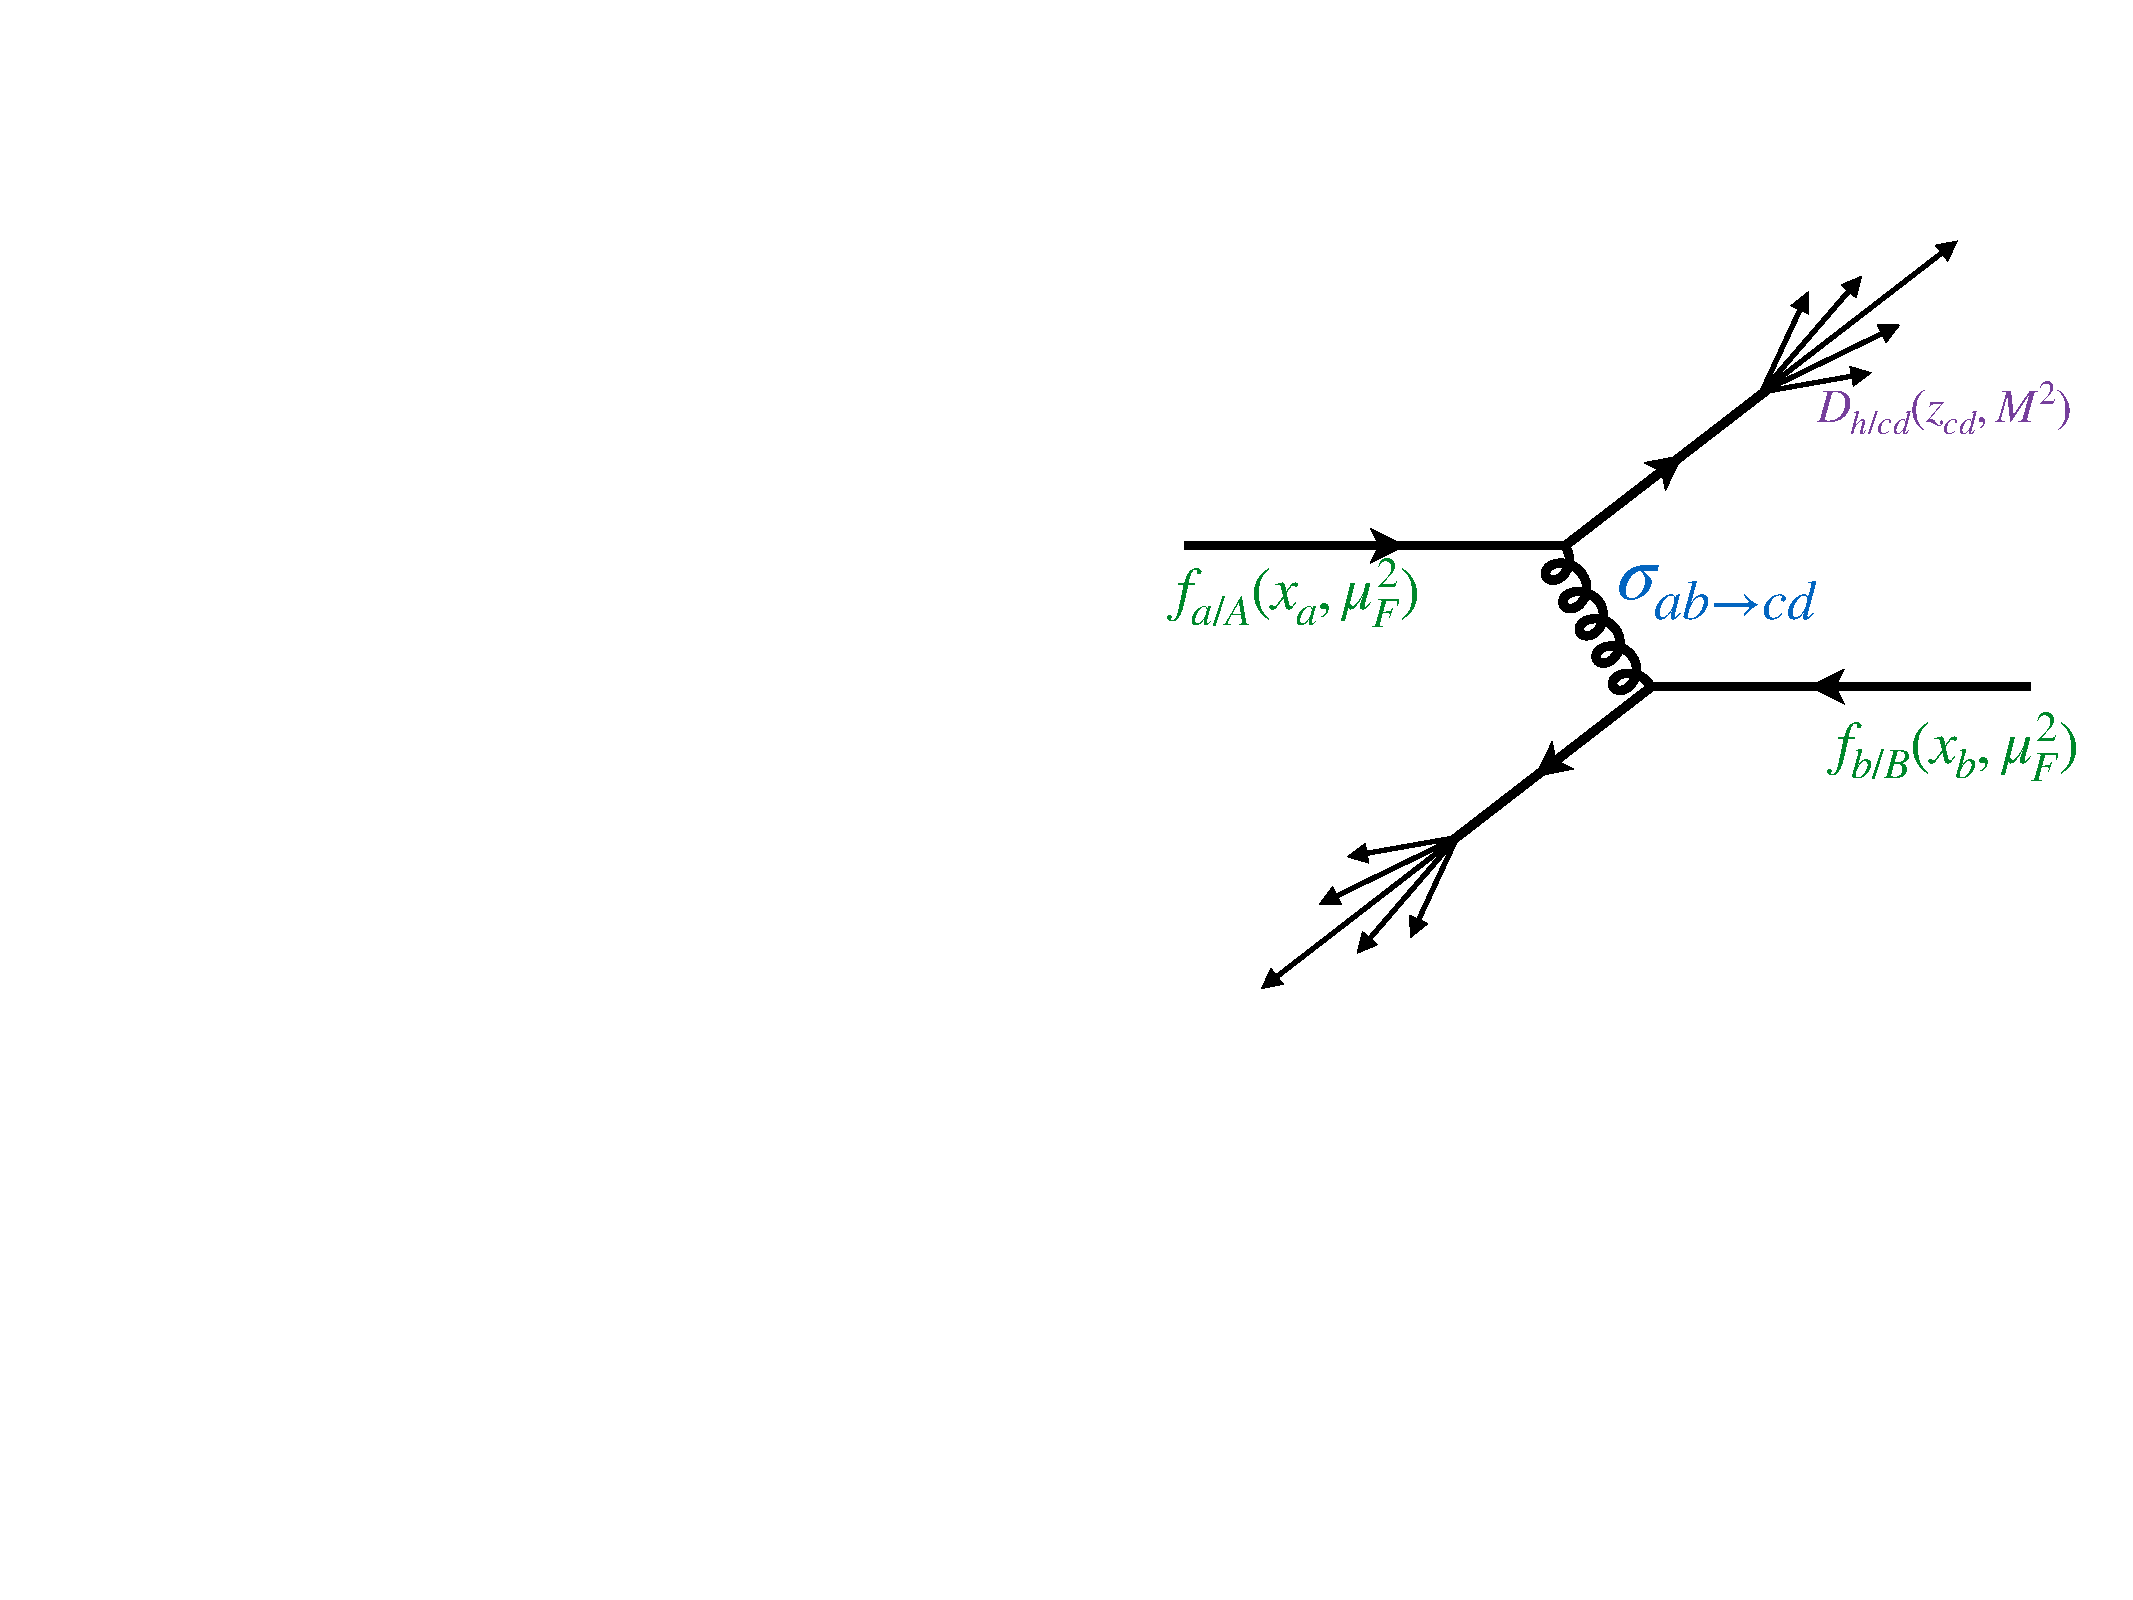
\includegraphics[width=0.35\textwidth]{figures/theory/feynman_jet}
\caption{Jet production from the process $pp \rightarrow hX$, factorizing in terms of the parton distribution functions, scattering cross sections, and jet fragmentation functions.}
\label{fig:feynman_jet}
\end{center}
\end{figure}

These processes can be described to leading order by perturbative QCD in terms of the parton distribution functions, scattering cross sections, and final state fragmentation functions as \cite{Qin:2015srf}:

\begin{align}
\label{eq:hadronCS}
d \sigma_{pp \rightarrow hX} \approx & \sum_{abjd} \int dx_a \int dx_b \int dz_j f_{a/p} (x_a, \mu_f) \otimes f_{b/p} (x_b, \mu_f) \\
& \otimes d\sigma_{ab\rightarrow jd} (\mu_f, \mu_F, \mu_R)  \nonumber \\
& \otimes D_{j \rightarrow h} (z_j, \mu_f) \nonumber
\end{align}
where $x_a = p_a/P_A, x_b = p_b / P_b$ are the initial momentum fractions carried by the interacting partons, $z_j = p_h / p_j$ is the momentum fraction carried by the final observed hadron.
$f_{a/p} (x_a, \mu_f)$ and $f_{b/p} (x_b, \mu_f)$ are the two parton distribution functions (PDFs), $d\sigma_{ab\rightarrow jd} (\mu_f, \mu_F, \mu_R)$ is the differential cross section for parton scattering and $D_{j\rightarrow }(z_j,\mu_F)$ is the fragmentation function (FFs) for parton $j$ to hadron $h$.
$\mu_f$ and $\mu_F$ are the factorization scales and $\mu_R$ is the renormalization scale.
These are typically taken to be the same hard scale $Q$, given by the hadron \pt.
The PDFs, measured via DIS experiments, characterize the initial state and represent the probability of finding a parton with longitudinal momentum fraction $x$ (shown in Figure~\ref{fig:bjorkenX}) in the initial hadron, while the FFs describe the probability of fragmenting to a hadron $h$ with given kinematic properties.

\begin{figure}[htbp]
\begin{center}
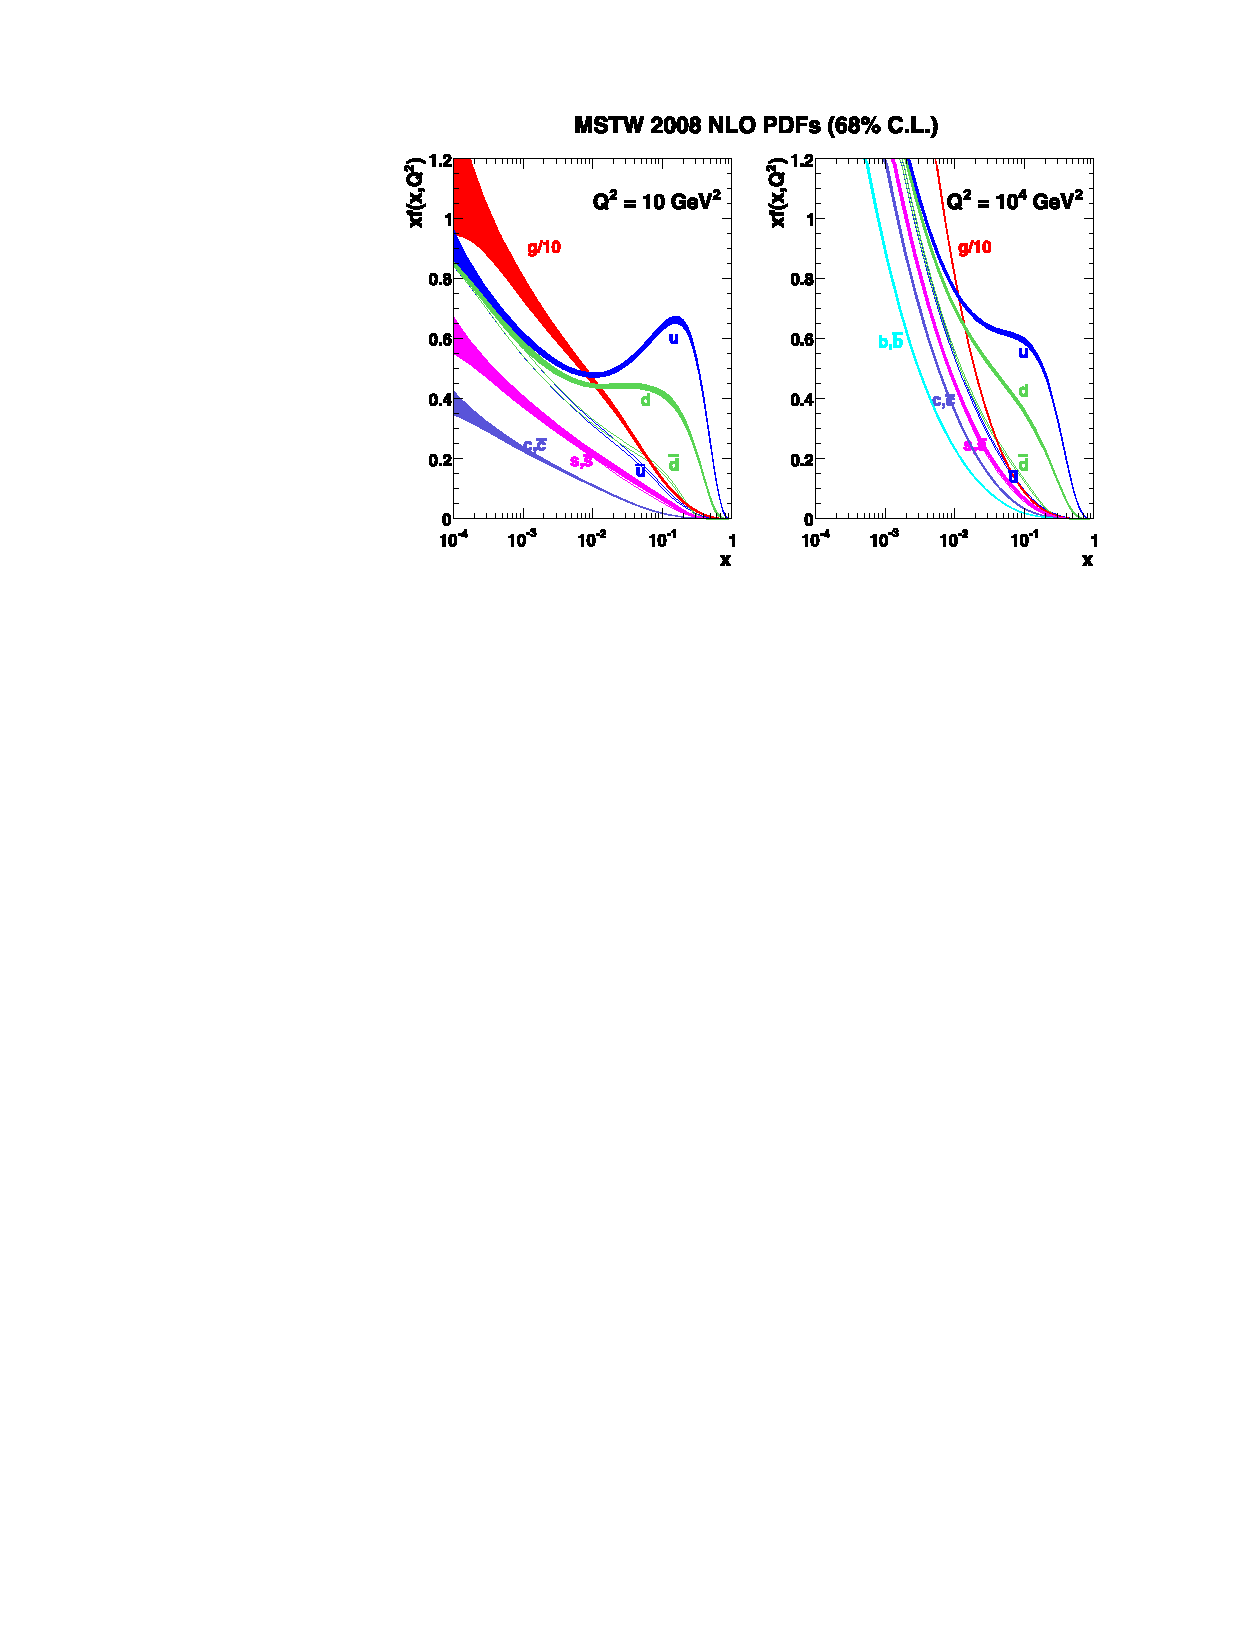
\includegraphics[width=0.65\textwidth]{figures/theory/bjorkenX}
\caption{The next to leading order (NLO) PDFs at (left) $Q^2 = 10 \mathrm{GeV}^2$ and (right) $Q^2 = 10^4 \mathrm{GeV}^2$.
The band is the associated one-sigma (68\%) confidence level uncertainty.
Figure from Ref.~\cite{Martin2009}.}
\label{fig:bjorkenX}
\end{center}
\end{figure}
 
The factorization of the jet production process is crucial because it allows for independently measuring and calculating the different components of the cross sections \cite{Majumder:2010qh}.
Jet cross sections in \pp\ and $p \bar{p}$ collisions measured by a variety of different experiments, and their comparison to theory calculations are shown in Figure~\ref{fig:jetcs}.
This in particular enables direct comparisons of jet observables in \pp\ collisions to those in heavy ion collisions and determine their modifications.
The fragmentation functions in \epm\ collisions in terms of collision energy \sqrts, and the scaled energy of the hadron $x$, are shown in Figure~\ref{fig:jetFrag}.

 \begin{figure}
\centering
\begin{subfigure}{.45\textwidth}
  \centering
  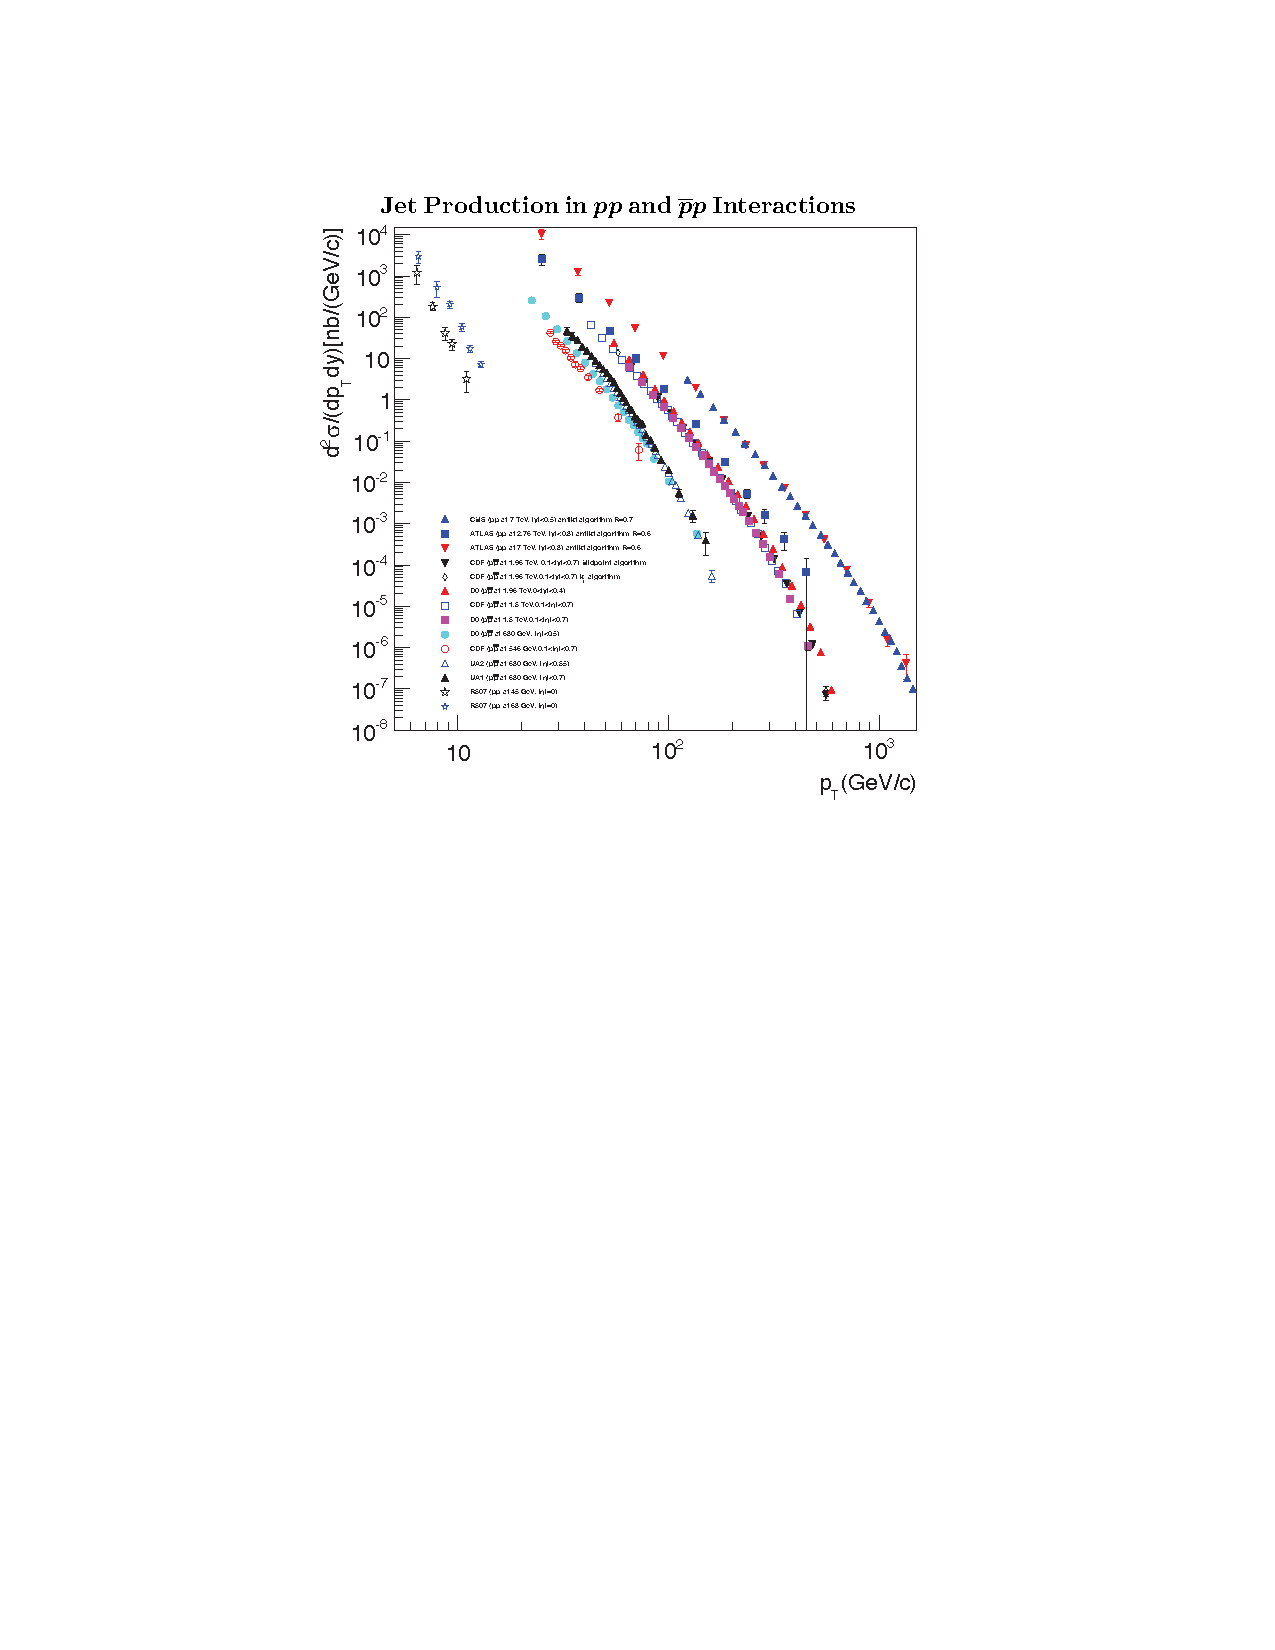
\includegraphics[width=\linewidth]{figures/theory/jetcs_pp}
  \caption{Inclusive differential jet cross sections shown as a function of jet transverse momentum from different experiments.
  Figure from Ref.~\cite{Olive_2016}.}
  \label{fig:jetcs_pp}
\end{subfigure}
\qquad  \qquad  
\begin{subfigure}{.45\textwidth}  
  \centering
  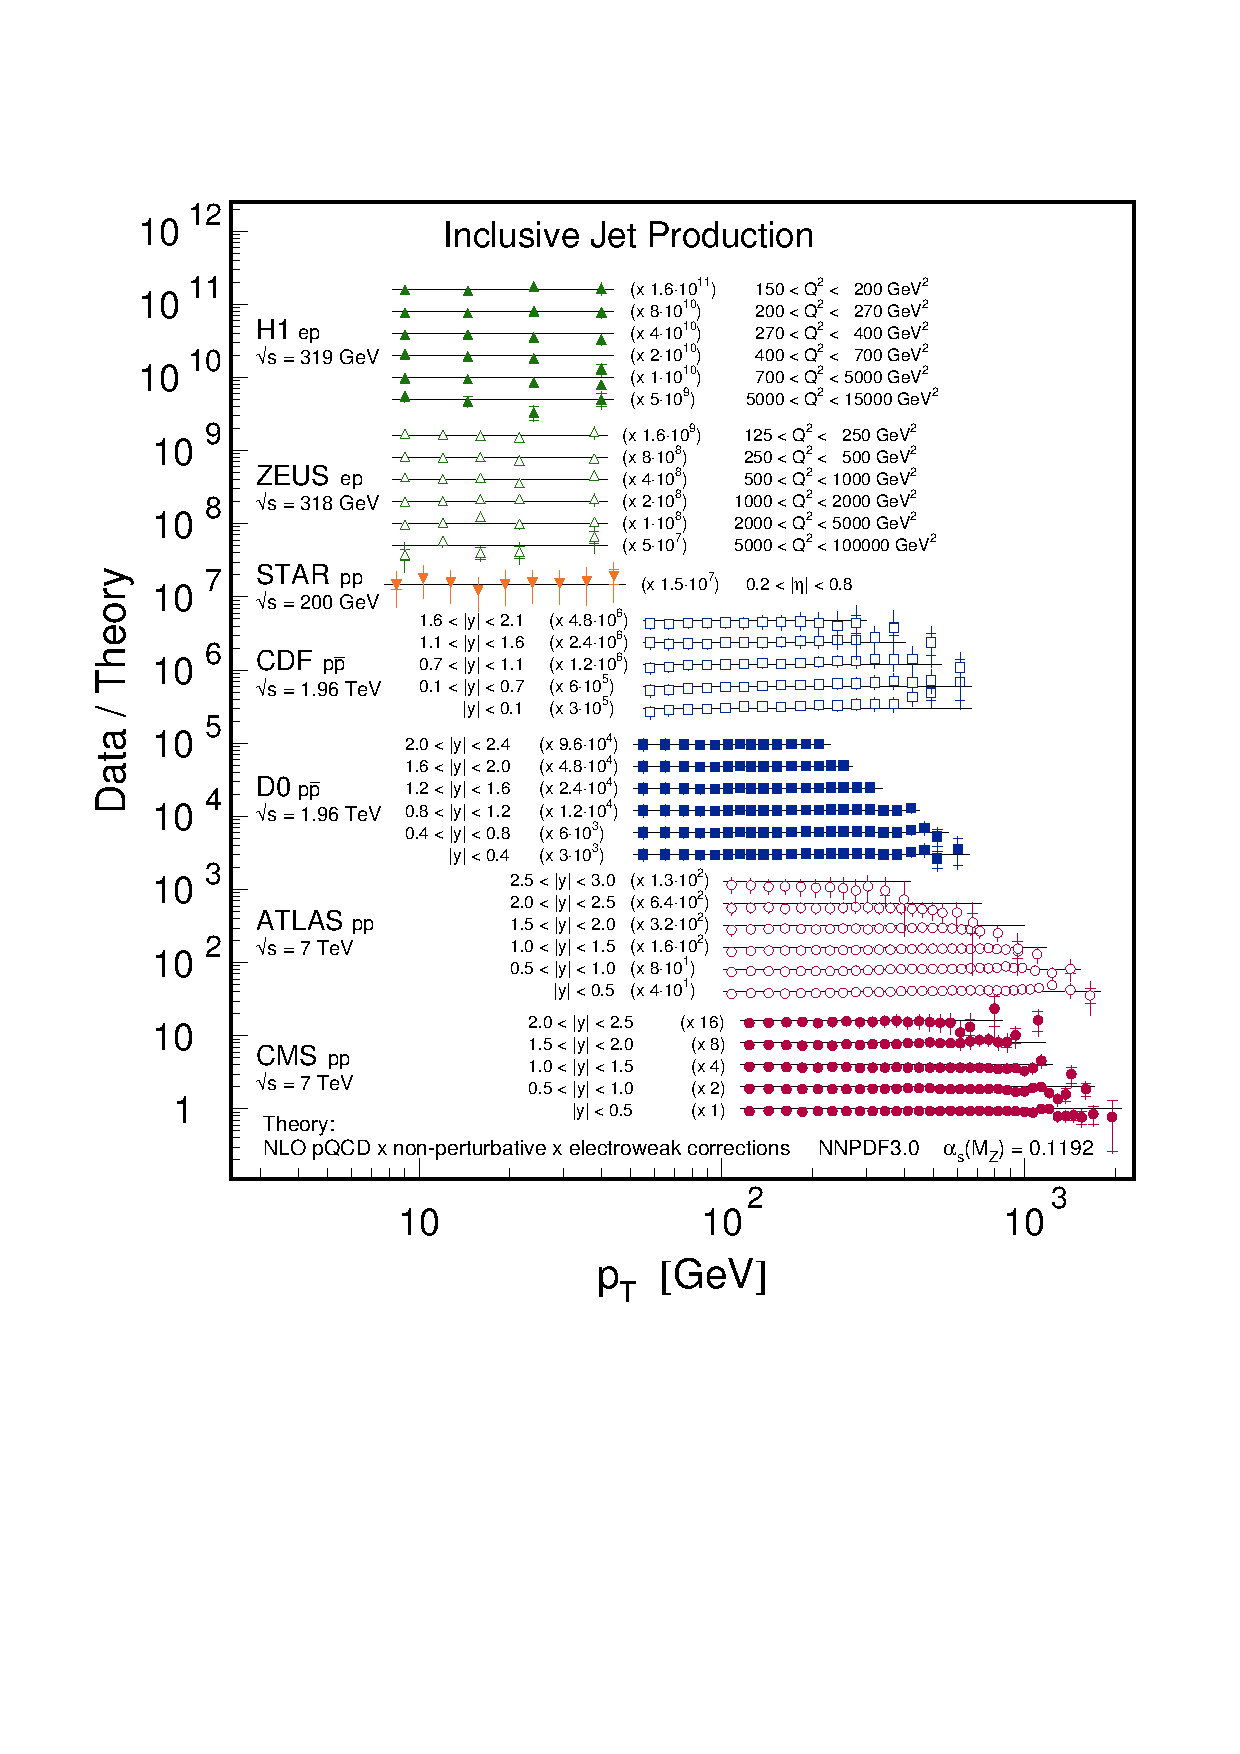
\includegraphics[width=\linewidth]{figures/theory/jetcs_pp_theory_comparison}
  \caption{Ratios of data over theory for some jet cross sections measured by different experiments.
  The next to leading order predictions are derived using the NNPDF3.0 PDF set.
  Figure from Ref.~\cite{Britzger:2017maj}.}
  \label{fig:jetcs_pp_theory_comparison}
\end{subfigure}
\caption{(Left) Some inclusive jet cross sections in data (left) and their comparison to theory (right).}
\label{fig:jetcs}
\end{figure}

\begin{figure}[htbp]
\begin{center}
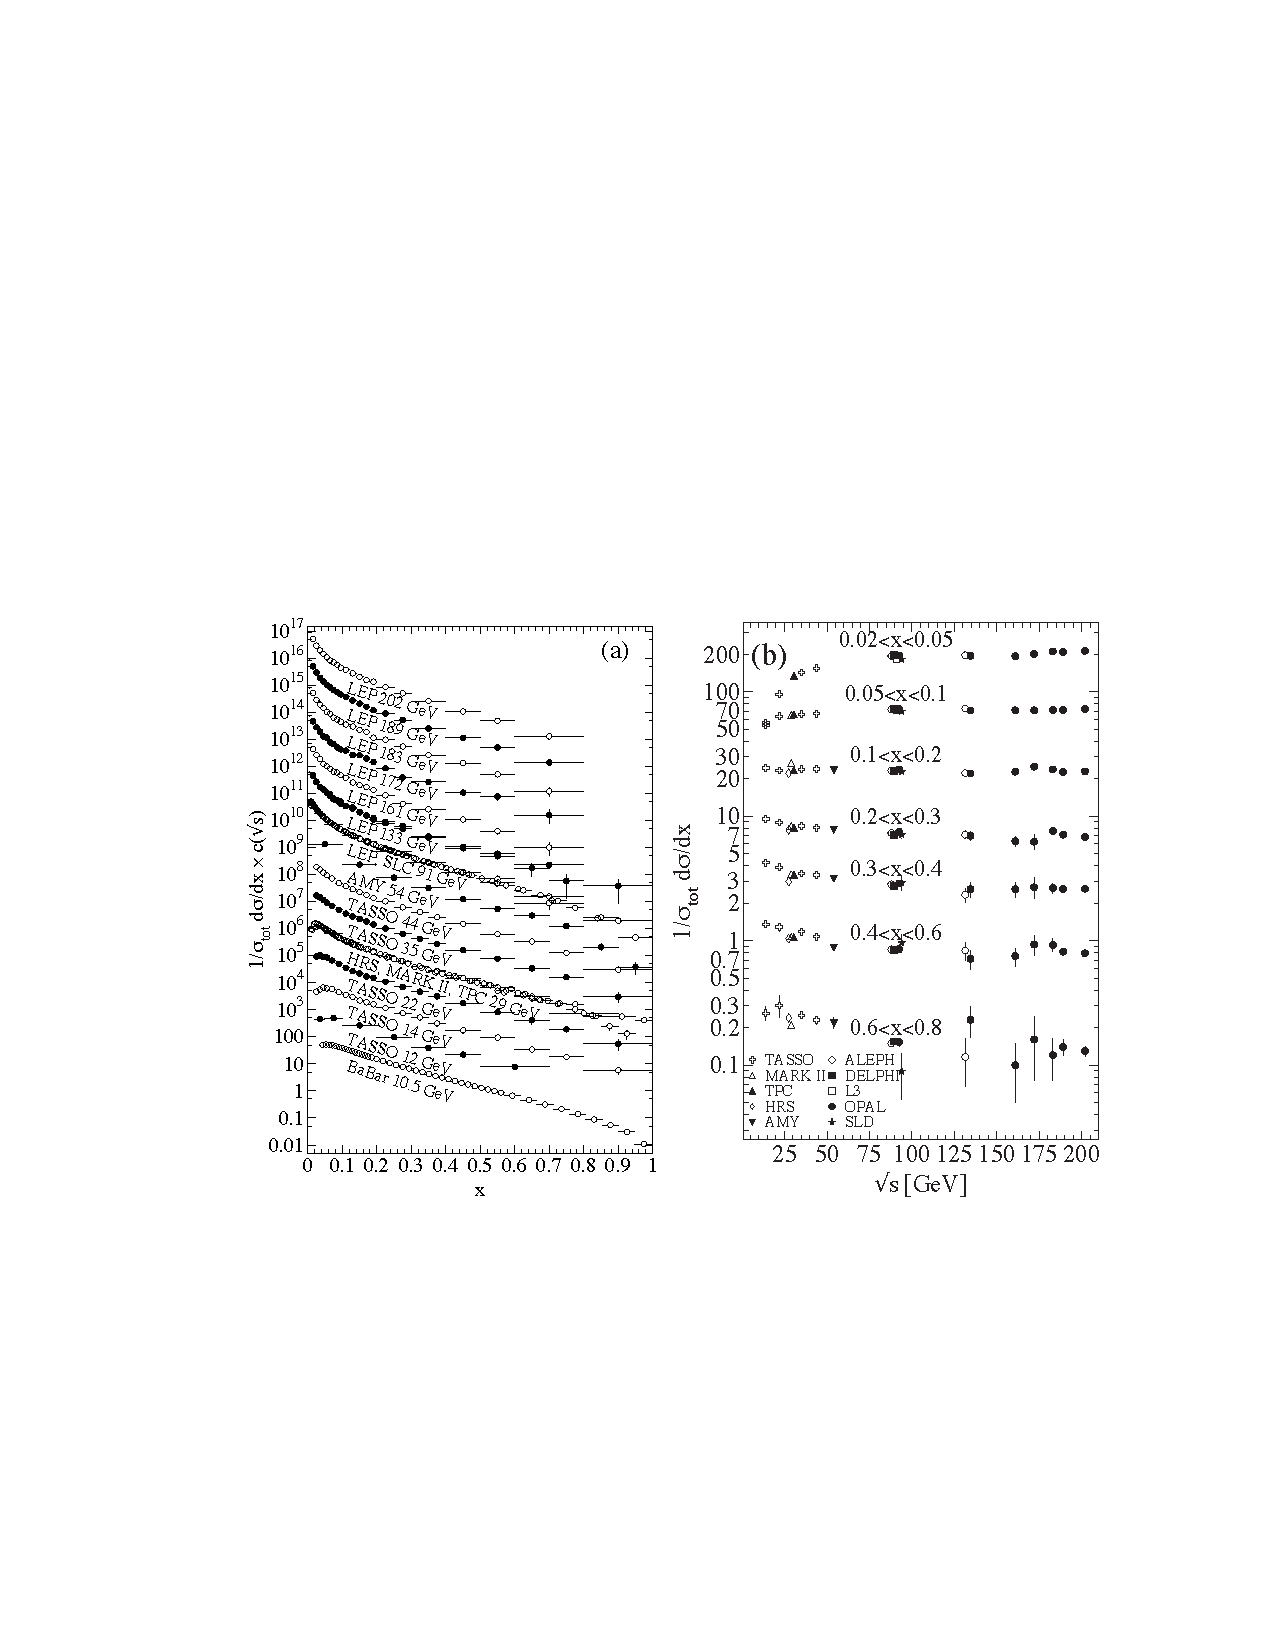
\includegraphics[width=0.75\textwidth]{figures/theory/jetFrag}
\caption{Measurements of the \epm\ fragmentation functions for (left) different center-of-mass energies as a function of $x$, and (right) for different ranges of $x$ as a function of \sqrts. The curves on the left are scaled for visibility. 
Figure from Ref.~\cite{PhysRevD.98.030001}.}
\label{fig:jetFrag}
\end{center}
\end{figure}




%%%%%%%%%%%%%%%%%%%%%%%%%%%%%%%%%%%%%
\subsection{Jets in heavy ion collisions}
%Both the PDFs and FFs are universal and their scale dependence evolves via the Dokshitzer-Gribov-Lipatov-Altarelli-Parisi (DGLAP) equations \cite{ALTARELLI1977298, Gribov:1972ri, Dokshitzer:1977sg}.
%These calculations can be compared to the inclusive charged particle distributions in \sqrts = 13 TeV \pp\ collisions and shown in Figure~\ref{fig:inclhadronCS}.
%The energy lost by a jet serves as further confirmation that the medium produced in a heavy ion collision is strongly coupled.

In the case of heavy ion collisions, after accounting for geometric scaling effects by the nuclear thickness function as mentioned in Section~\ref{sec:qgp_hi},  jet observables can be modified due to two sources: the nuclear PDF being distinct from a proton PDF, and the formation of the quark gluon plasma.
The former is collectively referred to as cold nuclear matter (CNM) effect, and can be quantified by defining a nuclear modification factor for the PDF:

\begin{align}
R_a^A (x, Q^2) = \frac{f_{a/A} (x, Q^2)}{f_{a/p}(x, Q^2)}
\end{align}
where $f_{a/A}$ and $f_{a/p}$ are the nuclear and proton PDFs respectively.
This $R_a^A$ factor is determined by global fits to data from DIS measurements \cite{PhysRevC.76.065207, PhysRevD.69.074028, Eskola_2009}.
CNM effects include the following contributions:
\begin{itemize}
\item Shadowing: This is a destructive interference effect that reduces the interactions of a nucleon incident on a nucleus within its interior and on its back face.
This effect reduces the effective number of nucleons in an inelastic interaction to $A^{2/3}$.
For $Q^2$ of the order of a few $\mathrm{GeV}^2$, this effect dominates for $x < 0.05$ and implies $R_a^A (x, Q^2) < 1$  \cite{PhysRevLett.64.1342}.
\item Anti-shadowing: This compensates for the shadowing effect based on the momentum sum rule, and for $Q^2$ of the order of a few $\mathrm{GeV}^2$ implies $R_a^A (x, Q^2) > 1$ over the region $0.05 < x < 0.20$.
\item EMC: The modification of the nuclear structure function was first observed by the European Muon Collaboration \cite{AUBERT1983275}.
Recent observations have suggested that the effect is caused by short-range correlated nucleon pairs within nuclei \cite{PhysRevC.85.047301}.
For $Q^2$ of the order of a few $\mathrm{GeV}^2$, this effect dominates for $0.2 < x < 0.80$ and implies $R_a^A (x, Q^2) < 1$.
\item  Fermi Motion: This effect considers the motion of the nucleons within the nucleus.
It results in $R_a^A (x, Q^2) > 1$  over the $x > 0.8$ region for $Q^2$ of the order of a few $\mathrm{GeV}^2$ \cite{Saito:1985ct}.
\end{itemize}

CNM effects are experimentally measured using $p+A$ systems where the size and shape of the plasma, and hence any effects thereof, are smaller.
Measurements of the jet nuclear modification factor in \pPb collisions, \RpPb, indicate that CNM effects are small for jets at all transverse momentum and pseudorapidity measured at the LHC \cite{2015392, Adam2016, Khachatryan2016b}.
This is shown in Figure~\ref{fig:RpPb}.
Energy densities in the \pbpb, \pPb, and \pp\ collision systems are shown in Figure~\ref{fig:pAenergyDensity}.

\begin{figure}[htbp]
\begin{center}
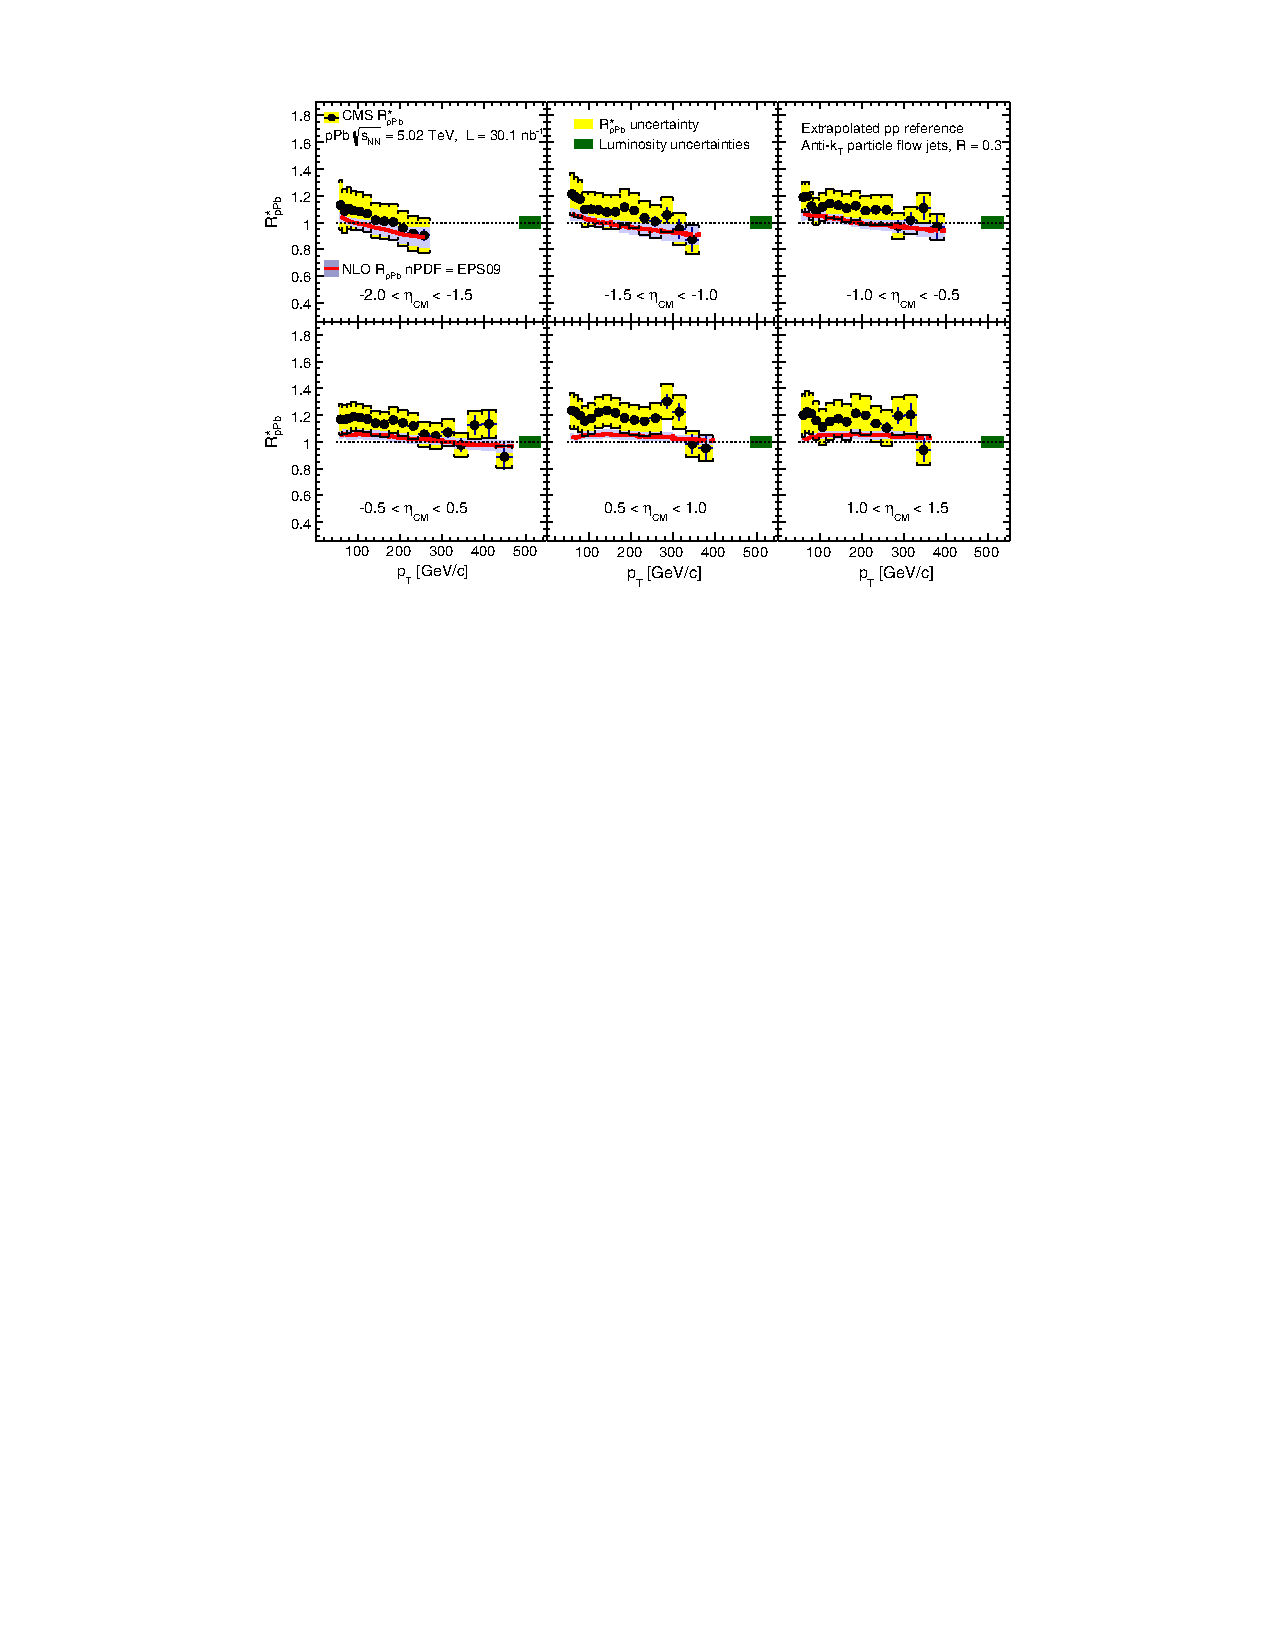
\includegraphics[width=0.75\textwidth]{figures/theory/RpPb}
\caption{The nuclear modification factor for jets in \pPb\ collisions as measured by CMS in different rapidity intervals.
Figure from Ref.~\cite{Khachatryan2016b}.}
\label{fig:pAenergyDensity}
\end{center}
\end{figure}



\begin{figure}[htbp]
\begin{center}
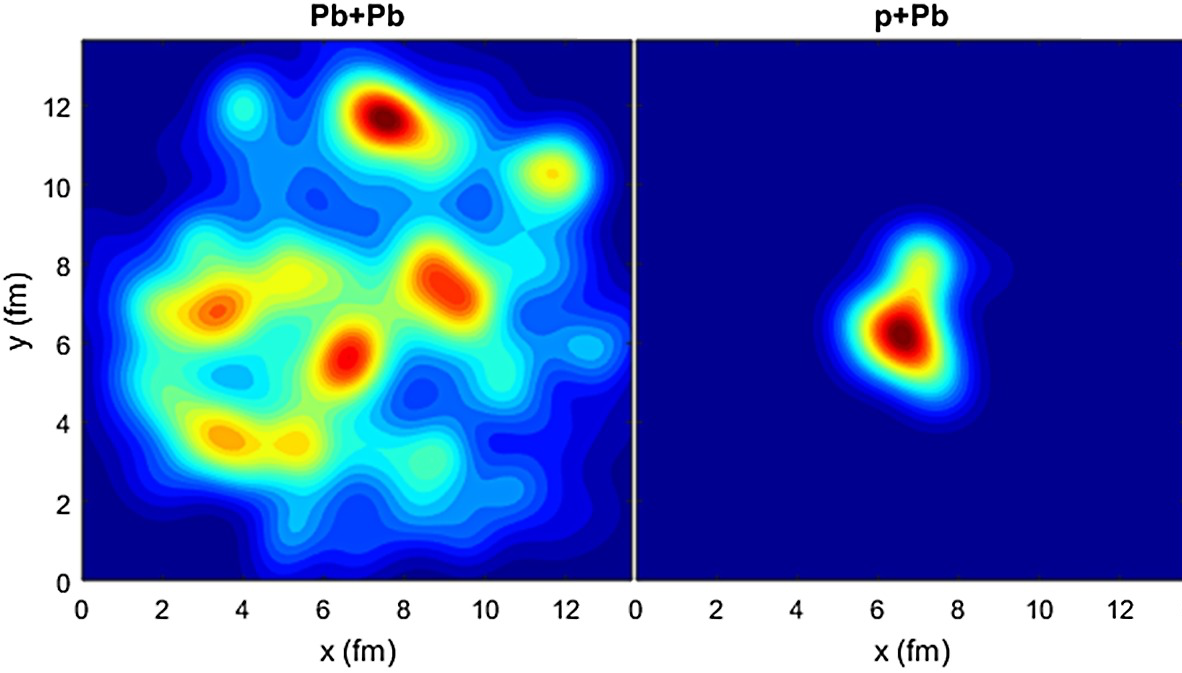
\includegraphics[width=0.85\textwidth]{figures/theory/everything_flows}
\caption{Snapshots of typical energy density profiles in (left) \pbpb, (middle) \pPb, and (right+far right) \pp\ collisions.
Figure from Ref.~\cite{Weller:2017tsr}.}
\label{fig:RpPb}
\end{center}
\end{figure}



The second source of modification is the formation of the hot and dense quark gluon plasma.
The hot nuclear matter effects further serve as an independent confirmation that the medium formed is strongly interacting.
Jets are formed early enough that they traverse the Quark Gluon Plasma and as strongly interacting particles, are both affected by, and affect the QGP.
This interaction typically results in the jet losing energy and forward momentum \cite{Chatrchyan:2012nia, 2019108}, with the lost energy being deposited in the medium \cite{Khachatryan2016}.
Jets can also pick up momentum transverse to the parton direction.
The hot nuclear matter effects can be considered to be a combination of collisional and radiative energy losses summarized in Figure~\ref{fig:jetEnergyLoss}.

\begin{figure}[htbp]
\begin{center}
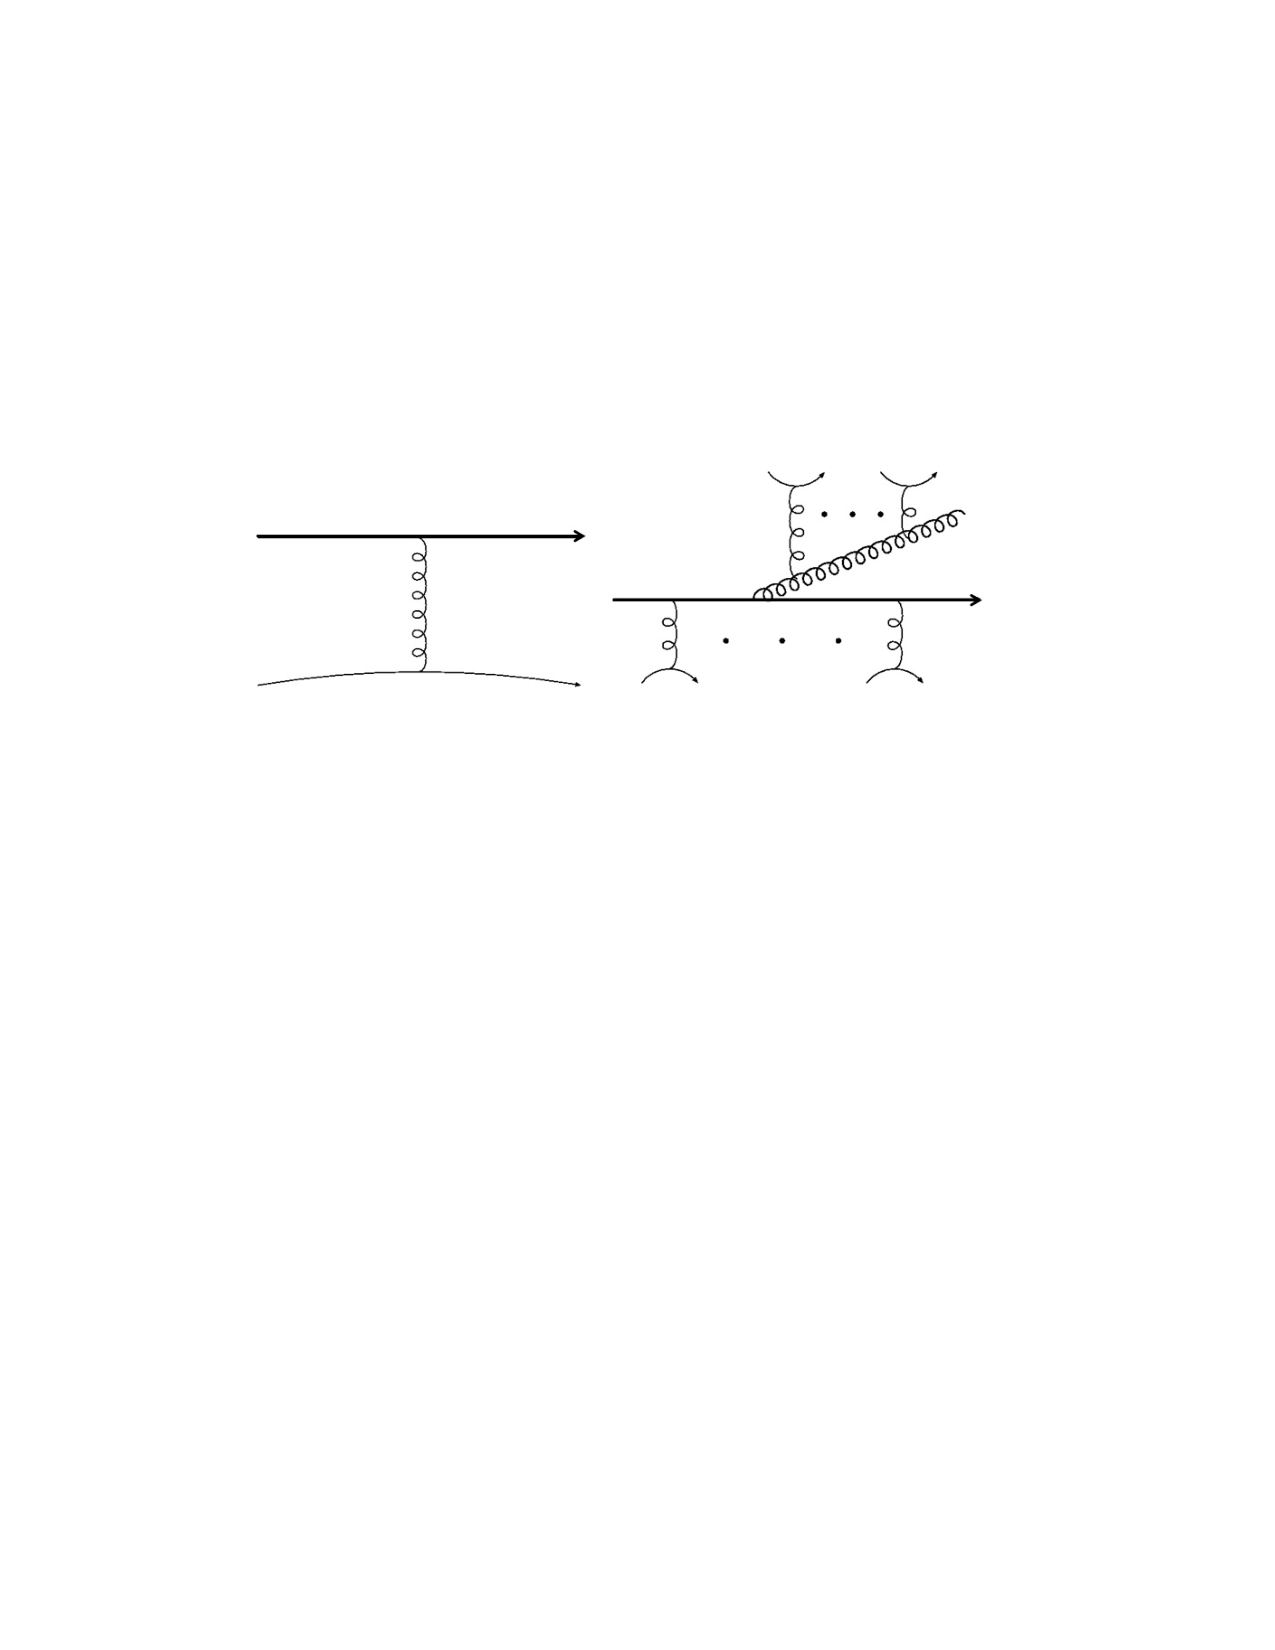
\includegraphics[width=0.75\textwidth]{figures/theory/jetEnergyLoss}
\caption{The typical diagrams for (left) collisional and (right) radiative energy losses for a parton in a hard scattering as it propagates through the QGP.
Figure from Ref.~\cite{Qin:2015srf}.}
\label{fig:jetEnergyLoss}
\end{center}
\end{figure}

\begin{itemize}
\item Collisional energy loss: This is a combination of elastic and inelastic collisions of the hard parton with the constituents of the quark gluon plasma.

\item Radiative energy loss: This is the larger source of parton energy loss and jet quenching.
These are modified by the presence of the plasma due to scatterings off of the plasma constituents.
A variety of radiative energy loss frameworks that have been developed include: Baier-Dokshitzer-Mueller-Peigne-Schiff-Zakharov (BDMPS-Z) \cite{BAIER1997291}, Gyulassy, Levai and Vitev (GLV) \cite{Gyulassy:1999zd}, Amesto-Salgado-Wiedemann (ASW) \cite{Wiedemann:2000za},  Arnold-Moore-Yaffe (AMY) \cite{Arnold:2001ba} and higher twist (HT) \cite{Guo:2000nz}.
\end{itemize}

Both hot and cold nuclear matter effects can be described by modifying Equation~\ref{eq:hadronCS} as:

\begin{align}
d \sigma_{AB \rightarrow hX}  \approx & \sum_{abjj'd} f_{a/A} (x_a) \otimes f_{b/B} (x_b) \\ 
& \otimes d\sigma_{ab\rightarrow jd} (\mu_f, \mu_F, \mu_R)  \nonumber \\
& \otimes P_{j\rightarrow j'} \nonumber \\
& \otimes D_{h \rightarrow j'} (z_j, \mu_f) \nonumber 
\end{align}
where the additional $P_{j\rightarrow j'}$ describes the interaction of the hard parton with the colored medium.
This is typically taken as part of the fragmentation modification as:

\begin{align}
\widetilde{D}_{h \rightarrow j'} (z_j, \mu_f) \approx \sum_{j'} P_{j\rightarrow j'} (p_{j'} | p_j) \otimes D_{h\rightarrow j'} (_{j'})
\end{align}




%%%%%%%%%%%%%%%%%%%%%%%%%%%%%%%%%%%%%%%%%%%%%%%
\subsection{Jet Algorithms}
\label{sec:jet_algo}
Jet algorithms map the momenta of final state particles into the momenta of jets, and form a core component of any jet measurement.
They can be broadly categorized as sequential recombination and cone algorithms~\cite{Atkin_2015}. 

Cone algorithms cluster particles in the $\eta-\phi$ space\footnote{The pseudorapidity $\eta = -\ln [\tan(\theta/2)]$ is related to the rapidity and is a spatial coordinate that describes the angle $\theta$ of a particle with respect to the beam axis. $\phi$ is the azimuthal angle around the beam axis. The The coordinate system of detectors is typically based on the $\eta-\phi$ plane.} assuming that the particles of a jet will be located in a conical region of the detector.
Some examples of cone algorithms are: iterative cone - progressive removal (IC-PR) \cite{ARNISON1983214}, iterative cone - split merge (IC-SM) \cite{Blazey:2000qt}, and SISCone \cite{Salam_2007}.

Sequential recombination algorithms on the other hand work by grouping particles in momentum space, with the result that they have fluctuating areas in $\eta-\phi$ space.
Some examples of these algorithms are: \kt\ \cite{Catani:1993hr}, \antikt\ \cite{Cacciari:2008gp}, and Cambridge/Aachen (C/A) \cite{Dokshitzer:1997in}.

Recombination algorithms have an advantage over the cone algorithms in that they are infrared and collinear safe (IRC).
This is related to instabilities in the cones that are found due to soft radiation.
In a collinear safe jet algorithm, the presence of a virtual loop or a collinear splitting of a central particle would not change the number of jets being reconstructed.
On the other hand, while a collinear unsafe jet algorithm would not change its output with the presence of a virtual loop, a splitting in the central particle would lead to the left and right most particles forming individual seeds, implying two reconstructed jets \cite{Salam:2009jx}.
Figure~\ref{fig:collinearSafe} describes the collinear safety problem.

\begin{figure}[htp]
\centering
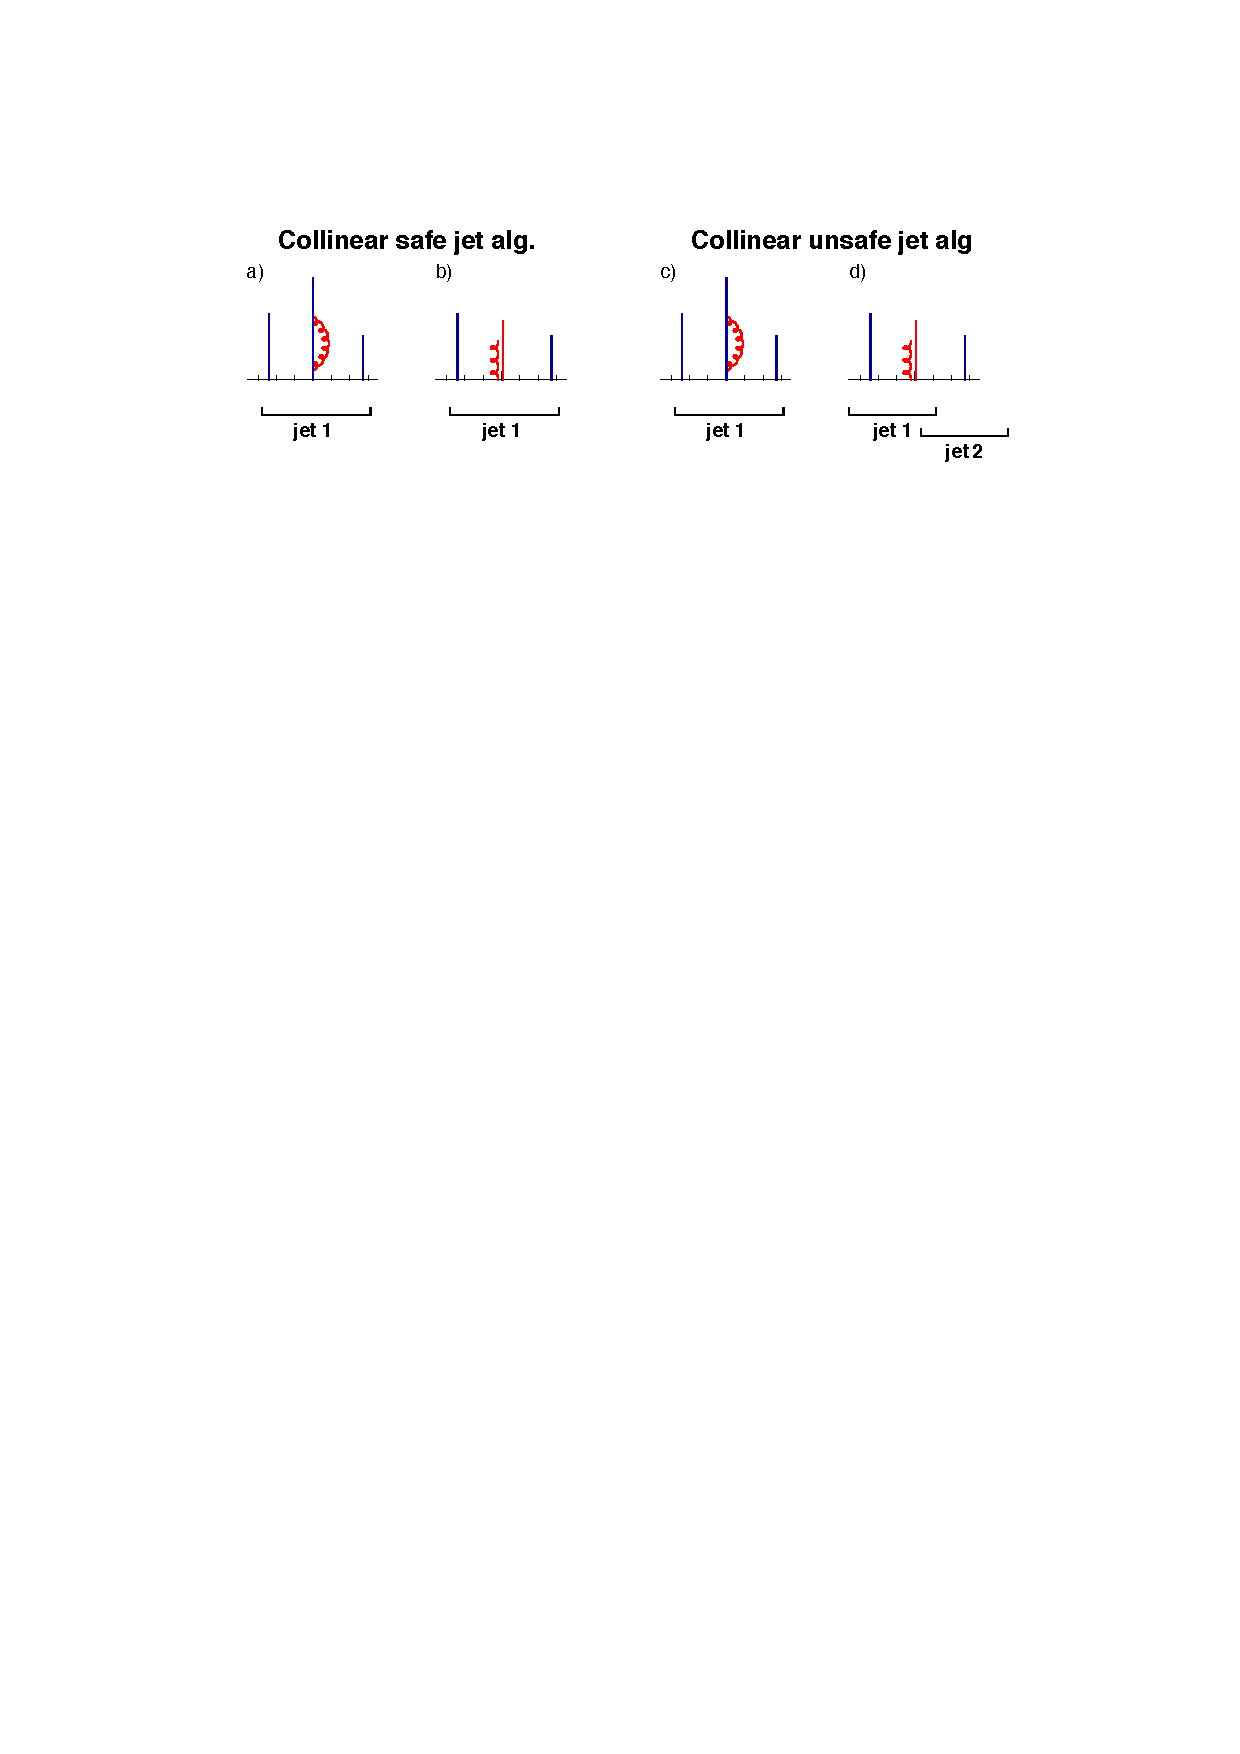
\includegraphics[width=.75\textwidth]{theory/collinearSafe}
\caption{An illustration of collinear unsafe behavior.
The particle \pt\ is proportional to the height and the horizontal axis indicates rapidity.
Figure from Ref.~\cite{Salam:2009jx}.}
\label{fig:collinearSafe}
\end{figure}

A schematic describing infrared safety problem is shown in Figure~\ref{fig:infraredSafe}.
Here an infrared safe algorithm would use the three particles as seeds iteratively find two stable cones.
An unsafe algorithm however would find three overlapping cones based on the addition of a soft seed.

\begin{figure}[htp]
\centering
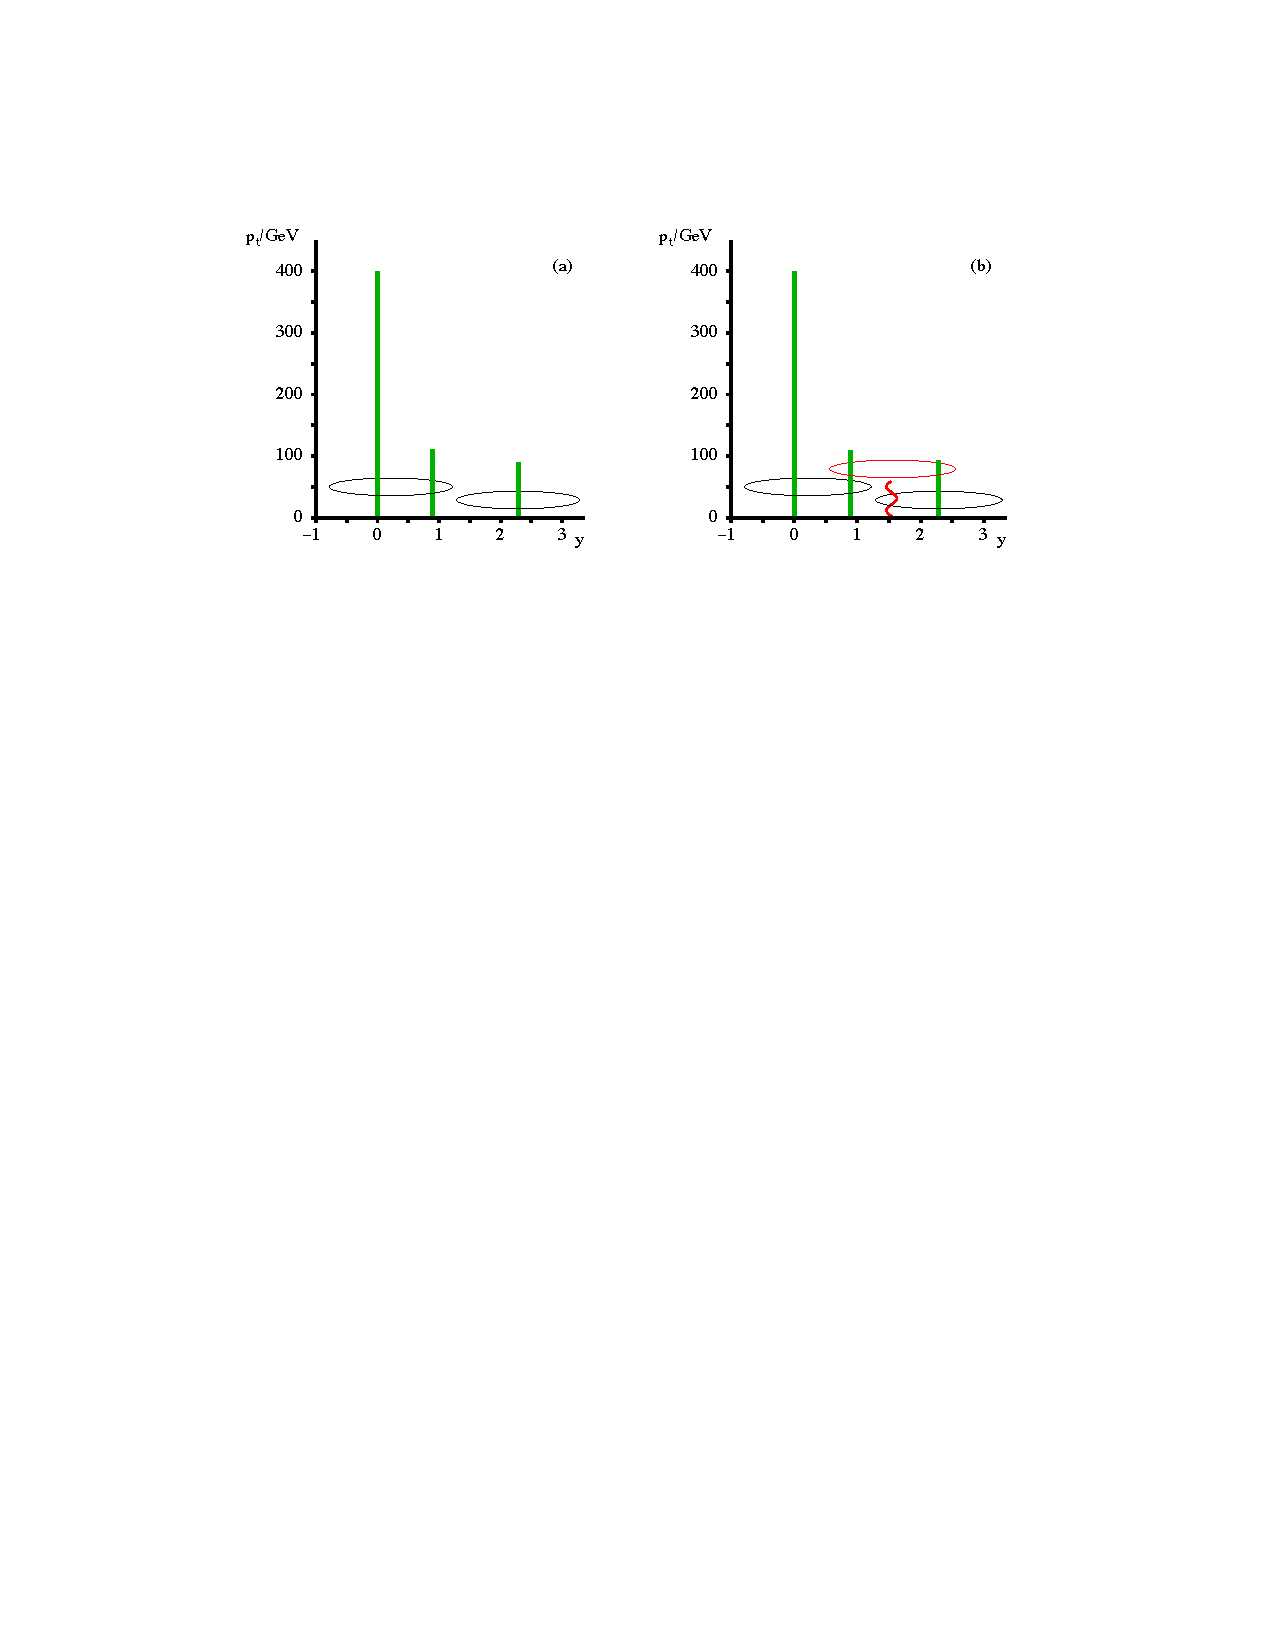
\includegraphics[width=.65\textwidth]{theory/infraredSafe}
\caption{An illustration of infrared unsafe behavior.
The particle \pt\ is proportional to the height and the horizontal axis indicates rapidity.
Figure from Ref.~\cite{Salam_2007}.}
\label{fig:infraredSafe}
\end{figure}

Sequential recombination algorithms are more popular because they are IRC safe and are discussed in further detail below. 
The general procedure for sequential recombination algorithms is as follows:
\begin{itemize}
\item Calculate all distances $d_{ij}$ between entities $i$ and $j$, and distance $d_{iB}$ between entity $i$ and beam $B$
\item Find the minimum of $d_{ij}$ and $d_{iB}$:
\begin{itemize}
\item If $d_{ij}$ is the minimum, combine $i$ and $j$ by summing their four-vectors, remove them from the list of particles and return to beginning.
\item If the smallest distance is $d_{iB}$, then take $i$ as the jet and remove it from the list of particles and return to beginning.
\end{itemize}
\item Continue the procedure till the list of items is empty.
\end{itemize}

In general the distance $d_{ij}$ between the objects is found the via the prescription

\begin{align}
d_{ij} &= \mathrm{min} (k_{Ti}^{2p} , k_{Tj}^{2p}) \frac{\Delta_{ij}^2}{R^2}  \\
d_{iB} &= k_{Ti}^{2p}
\end{align}
where $k_{Ti}$ is the transverse momentum of particle $i$ and $\Delta_{ij} = \sqrt{\Delta\eta_{ij}^2 + \Delta\phi_{ij}^2}$ is the distance between particles $i$ and $j$ in $\eta-\phi$ space.
$R$ the distance parameter and reflects the size of the jet being considered.

Different recombination algorithms use different values of $p$. 
The \kt\ algorithm has $p = 2$.
This results in clustering soft particles first, with the final jet having a fluctuating area.
This algorithm is susceptible to processes that contribute particles that do not belong to a jet.
The C/A algorithm uses $p = 0$.
This results in the distances between particles being completely independent of momentum. 
The \antikt\ algorithm uses $p = -1$.
Hence, the algorithm clusters hard particles first, making it the least susceptible to background. 
The behavior of the different clustering algorithms is shown in Figure~\ref{fig:JetClustering}.
The \antikt\ algorithm is the default used in all LHC collaborations.

\begin{figure}[htp]
\centering
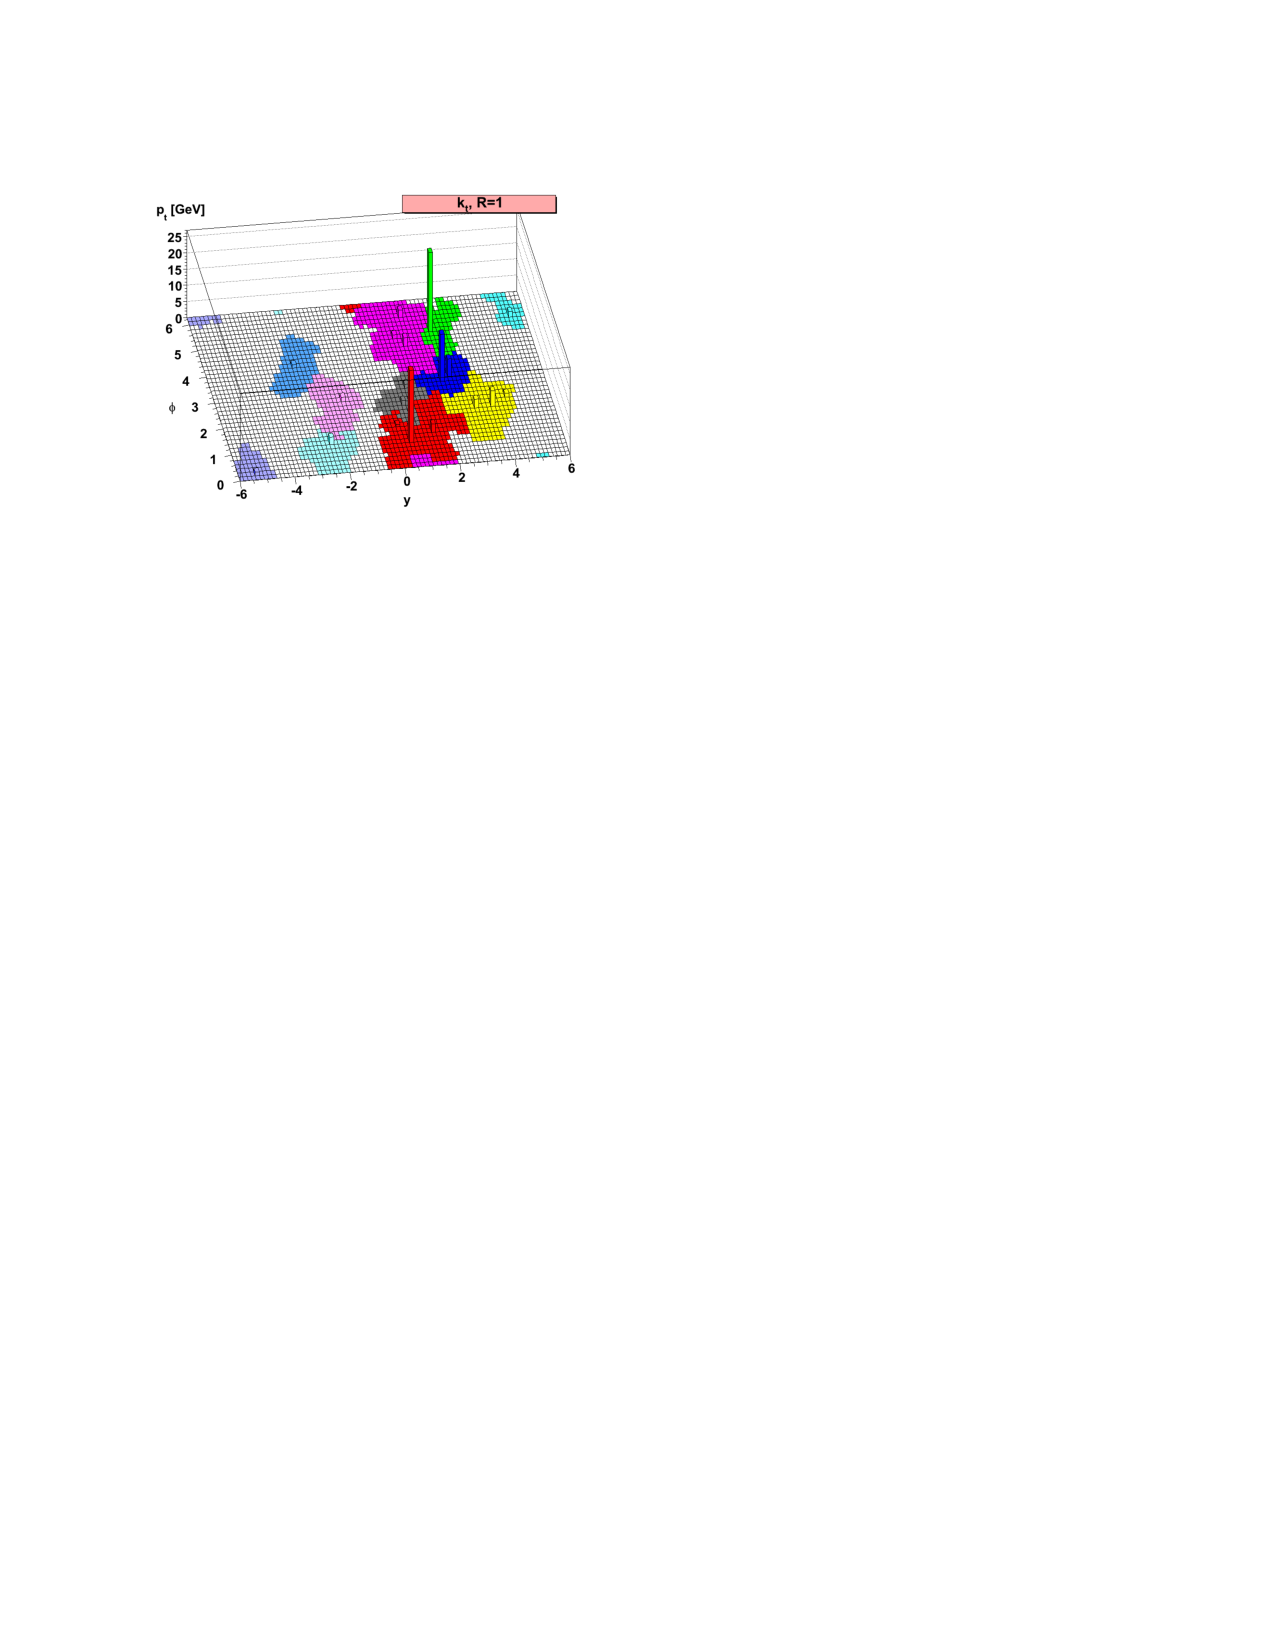
\includegraphics[width=.3\textwidth]{theory/jetReco_kt}\hfill
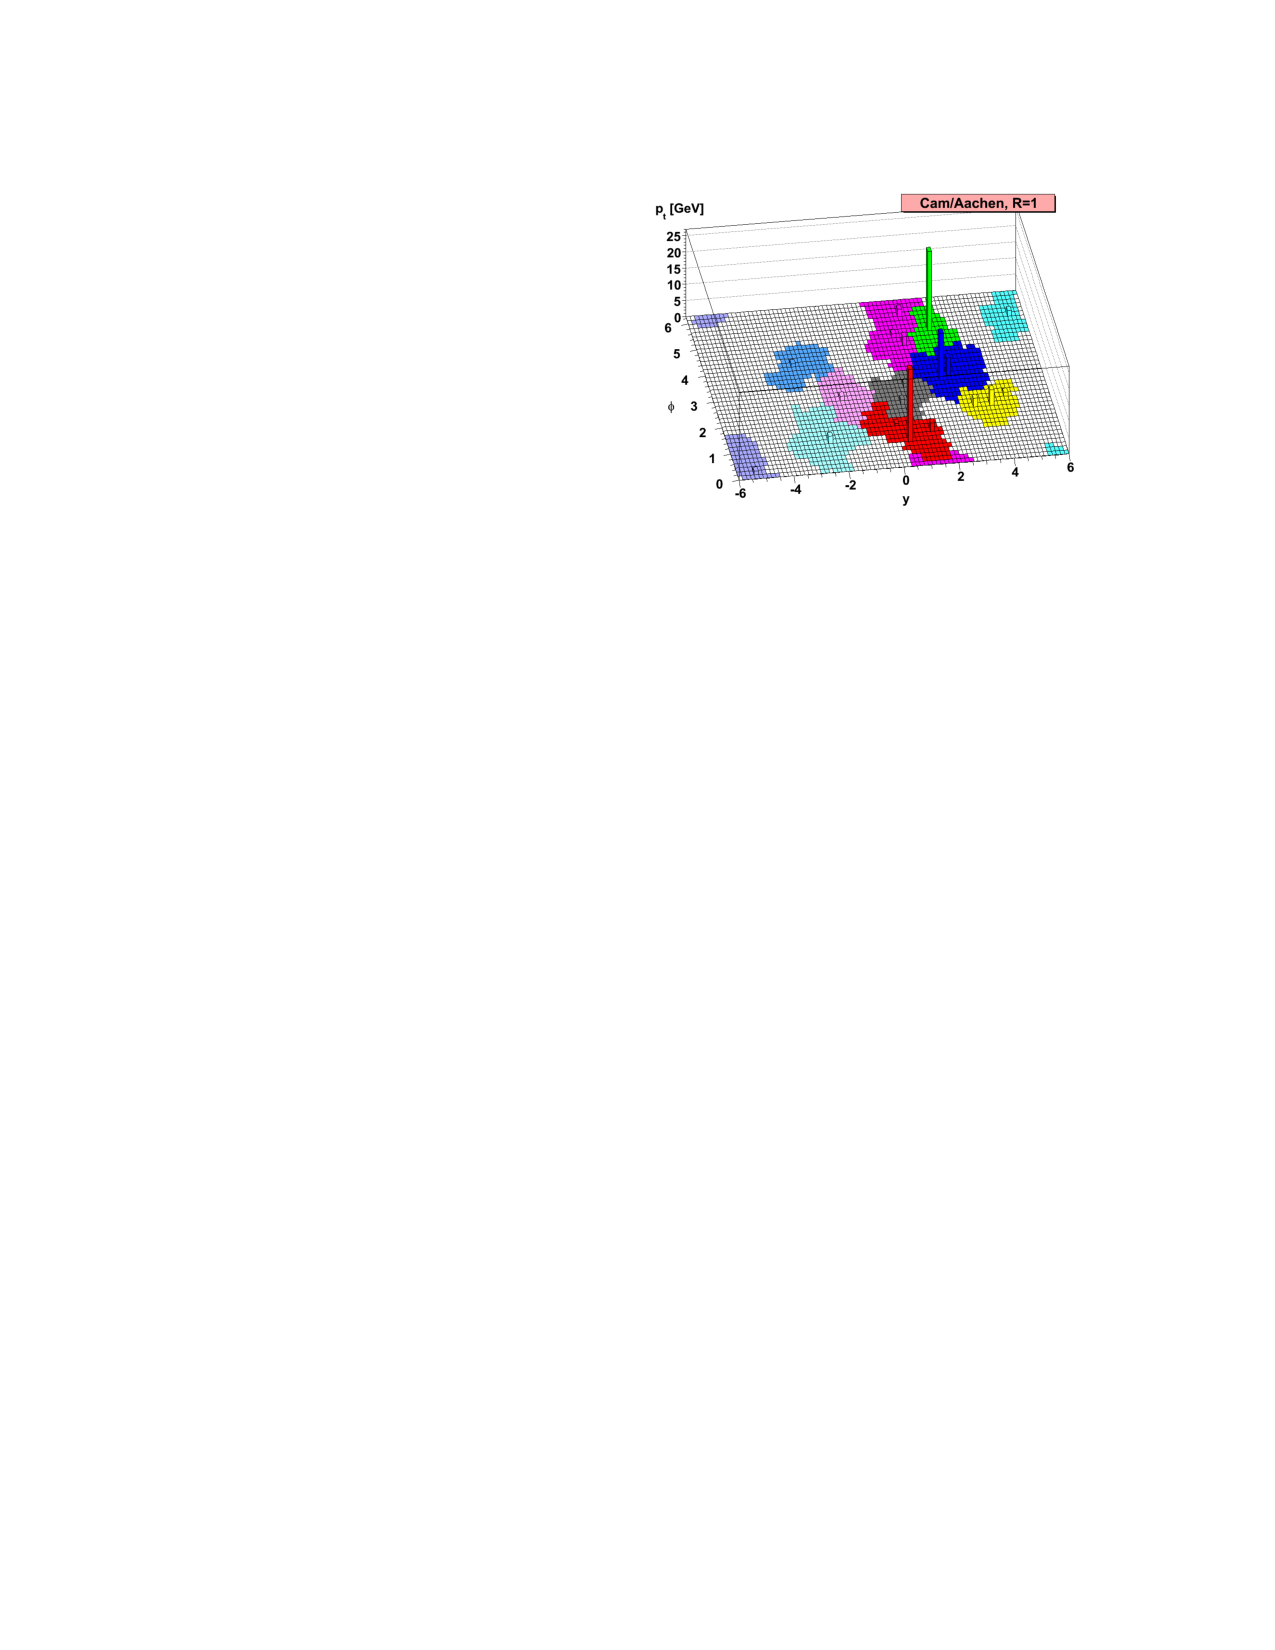
\includegraphics[width=.3\textwidth]{theory/jetReco_CA}\hfill
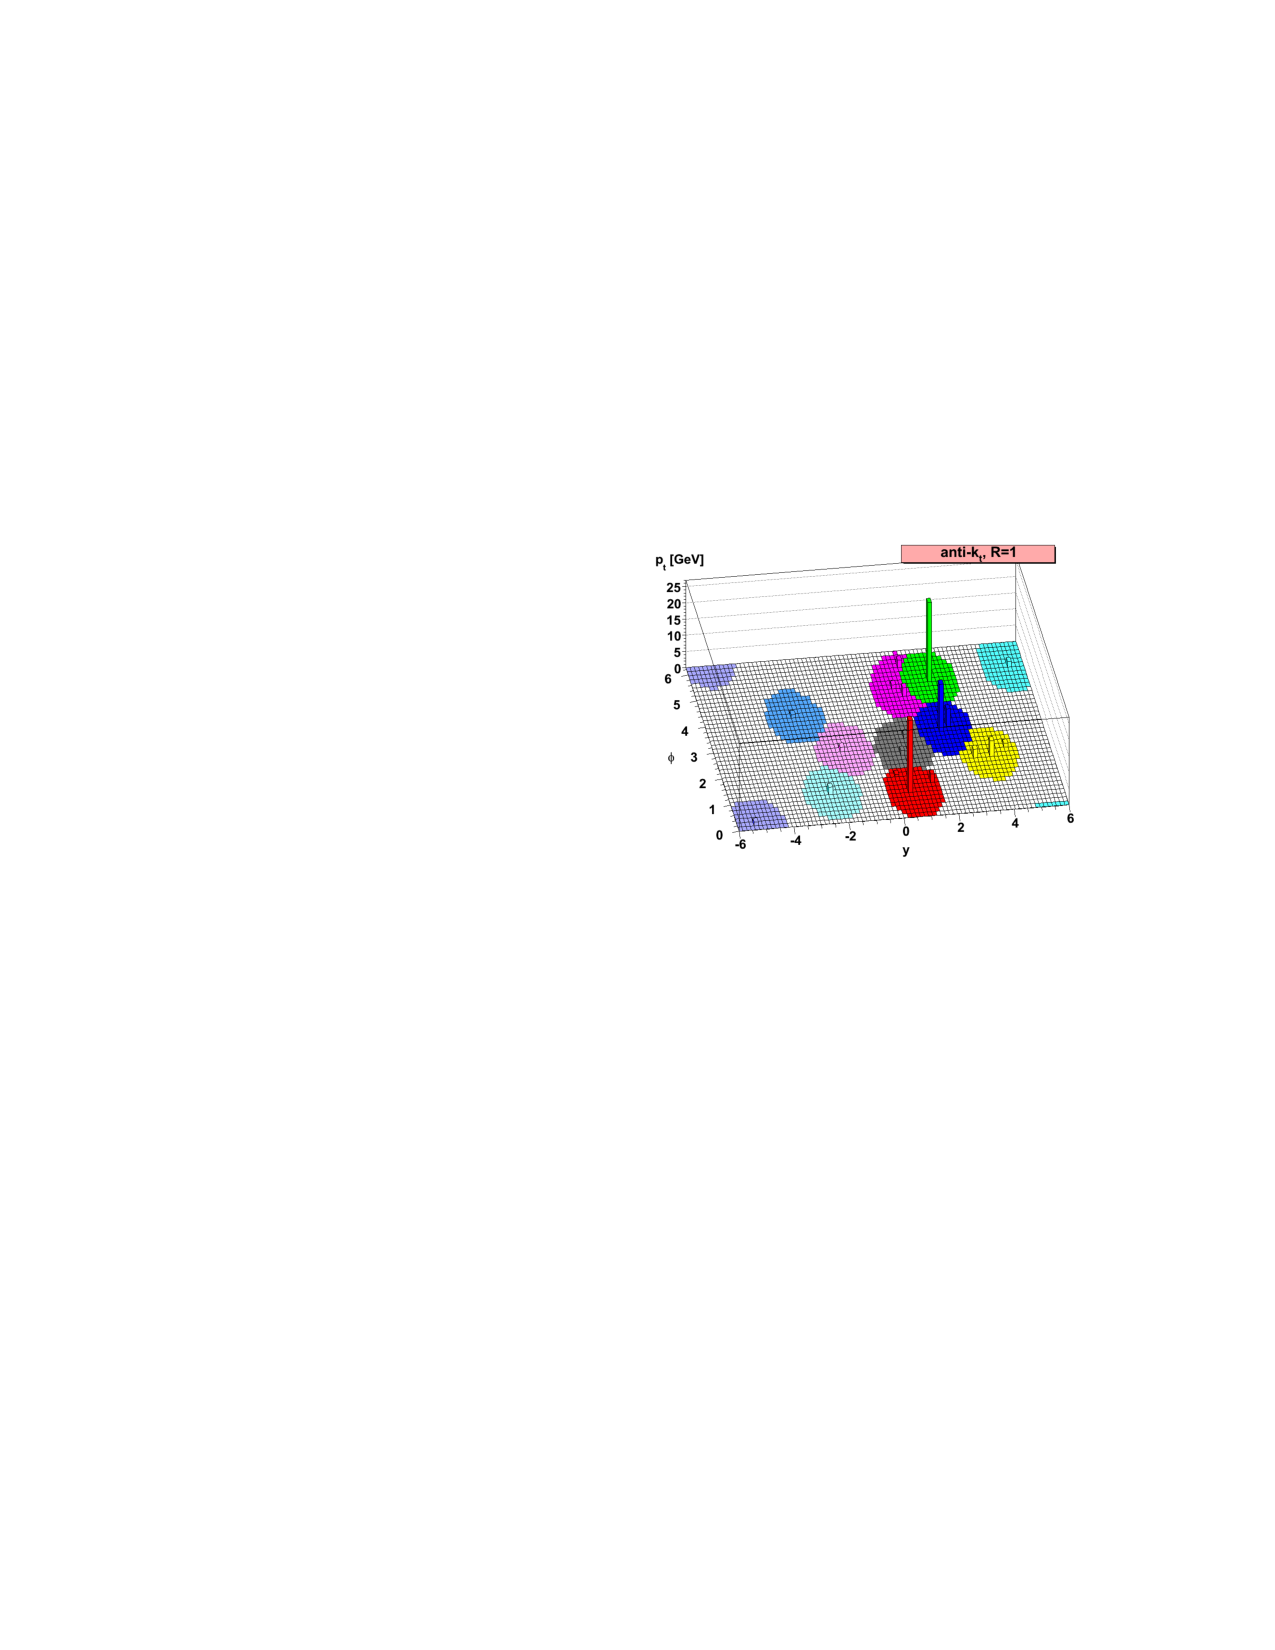
\includegraphics[width=.3\textwidth]{theory/jetReco_antikt}\hfill
\caption{Different clustering algorithms applied to the sample parton-level event.
Figures from Ref.~\cite{Cacciari:2008gp}.}
\label{fig:JetClustering}
\end{figure}



%The popularity of the \antikt\ algorithm comes from its overcoming of two common problems: collinear and infrared safety.
% the \antikt\ reconstruction algorithm is used with the distance parameter $R=0.4$
%A few jet measurements and their modifications by the presence of the Quark Gluon Plasma are discussed in Section~\ref{sec:jetMeasurements}.
%
%  jet cross section in  \sqrts = 13 TeV \pp\ collisions can be seen in Figure~\ref{fig:incljetCS}
%
%\begin{figure}[htbp]
%\begin{center}
%\includegraphics[width=0.55\textwidth]{figures/theory/incljetCS}
%\caption{The inclusive jet cross section as a function of \pt\ and $|y|$ as measured by ATLAS.
%The data are compared to NLO pQCD calculations.
%Taken from Ref.~\cite{Aaboud:2017wsi}.}
%\label{fig:incljetCS}
%\end{center}
%\end{figure}
%
%\begin{figure}[htbp]
%\begin{center}
%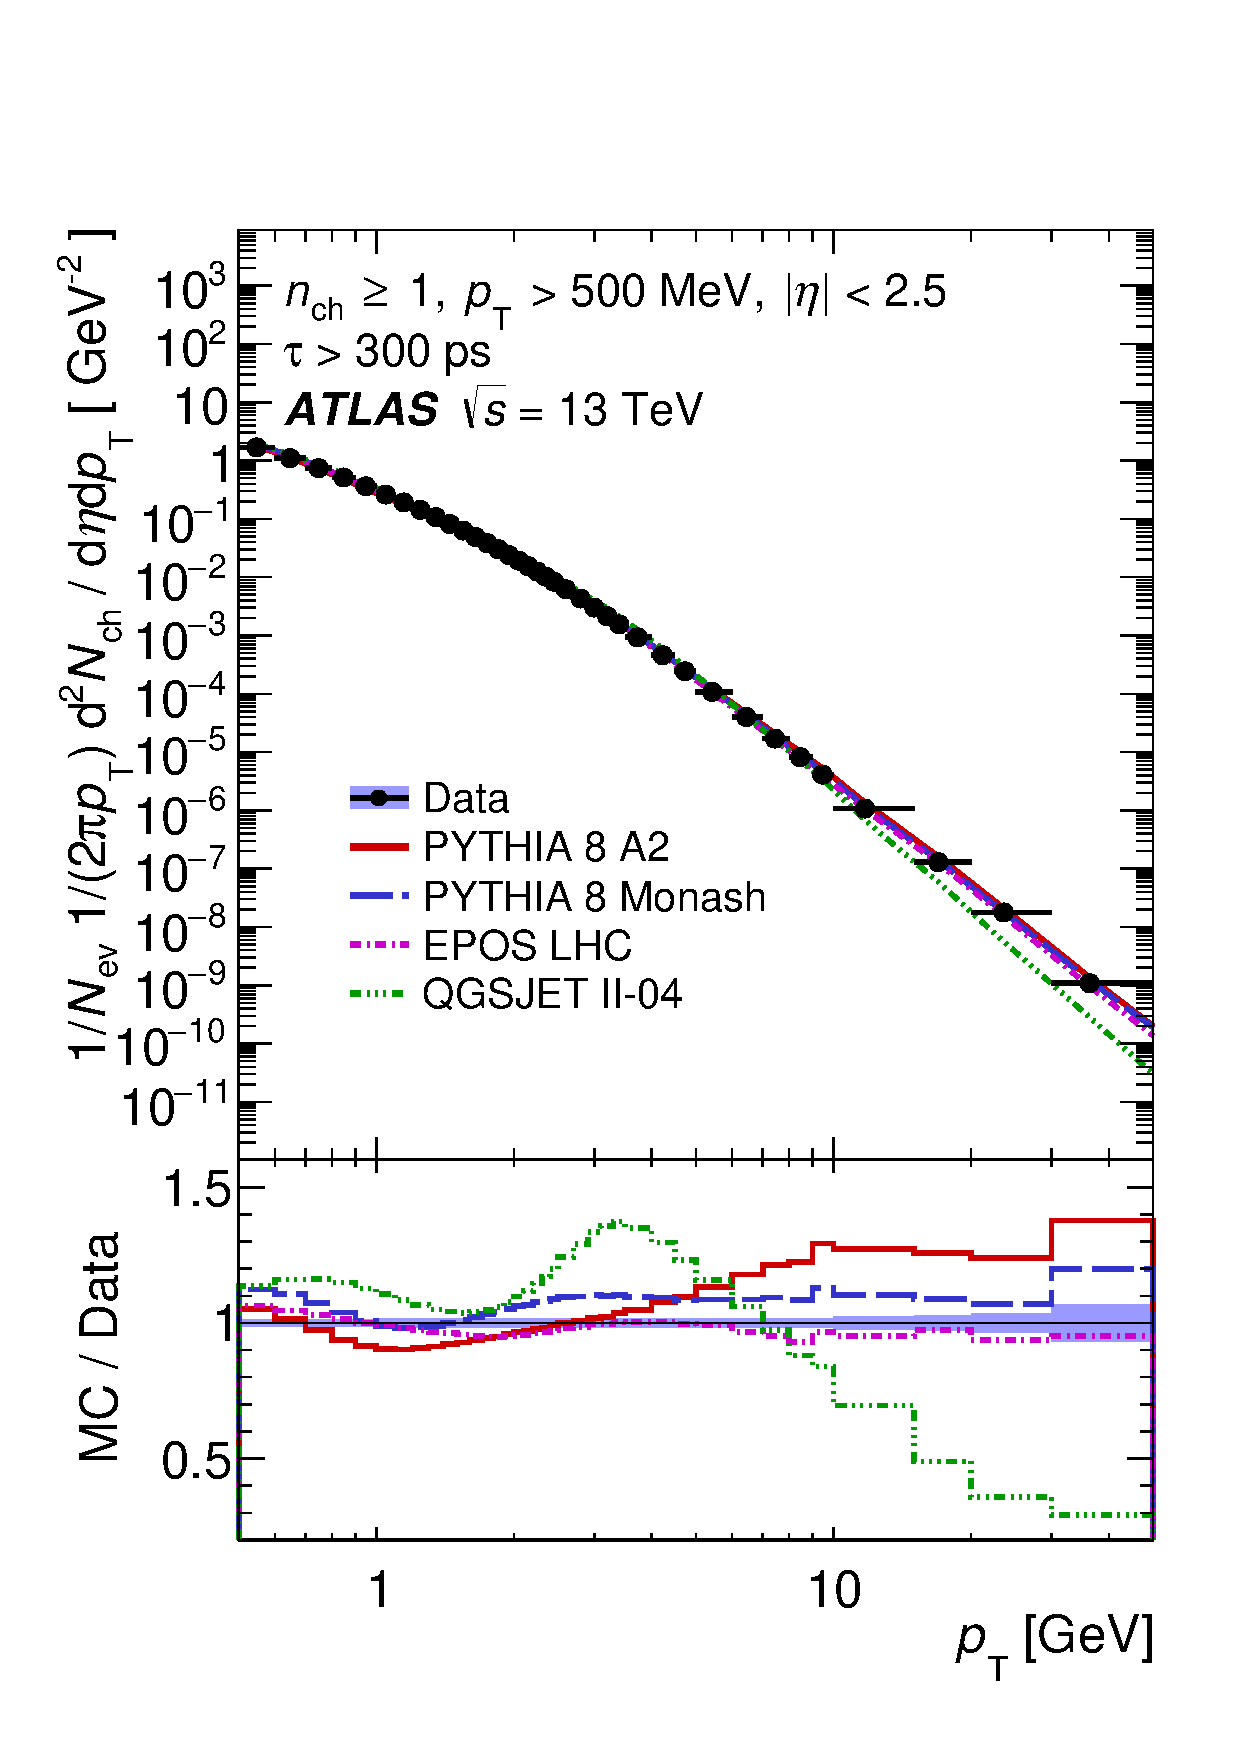
\includegraphics[width=0.55\textwidth]{figures/theory/inclhadronCS}
%\caption{The charged particle multiplicities as a function of transverse momentum \pt\ in \sqrts = 13 TeV \pp\ collisions as measured by ATLAS.
%The data are compared to NLO pQCD calculations.
%Taken from Ref.~\cite{201667}.
%}
%\label{fig:inclhadronCS}
%\end{center}
%\end{figure}
%
%Equation~\ref{eq:hadronCS} is written at leading order (LO) and includes contributions from $2\rightarrow2$ cross sections, LO re-summed PDFs and FFs, and single loop expression for the strong coupling \alphas.
%At next to leading order (NLO), the contributions from real $2\rightarrow3$ and virtual $2\rightarrow3$ processes, as well as the double loop expression for \alphas are included.
%These calculations describe the inclusive and pQCD, NLO calculations have next to leading order (NLO) calculations that include Figure~\ref{fig:incl_hadron_CS} hows the inclusive jet cross section as measured by ATLAS in \sqrts = 13 TeV \pp\ collisions.
%
%In a heavy ion collision where the QGP is formed, the hard scattering interactions between the partons strongly interact with the QGP due to their color charge and are modified and lose energy via collisions with the medium constituents, or gluon bremsstrahlung.
